\documentclass[12pt]{report}\usepackage[]{graphicx}\usepackage[dvipsnames]{xcolor}
% maxwidth is the original width if it is less than linewidth
% otherwise use linewidth (to make sure the graphics do not exceed the margin)
\makeatletter
\def\maxwidth{ %
  \ifdim\Gin@nat@width>\linewidth
    \linewidth
  \else
    \Gin@nat@width
  \fi
}
\makeatother

\definecolor{fgcolor}{rgb}{0.345, 0.345, 0.345}
\newcommand{\hlnum}[1]{\textcolor[rgb]{0.686,0.059,0.569}{#1}}%
\newcommand{\hlstr}[1]{\textcolor[rgb]{0.192,0.494,0.8}{#1}}%
\newcommand{\hlcom}[1]{\textcolor[rgb]{0.678,0.584,0.686}{\textit{#1}}}%
\newcommand{\hlopt}[1]{\textcolor[rgb]{0,0,0}{#1}}%
\newcommand{\hlstd}[1]{\textcolor[rgb]{0.345,0.345,0.345}{#1}}%
\newcommand{\hlkwa}[1]{\textcolor[rgb]{0.161,0.373,0.58}{\textbf{#1}}}%
\newcommand{\hlkwb}[1]{\textcolor[rgb]{0.69,0.353,0.396}{#1}}%
\newcommand{\hlkwc}[1]{\textcolor[rgb]{0.333,0.667,0.333}{#1}}%
\newcommand{\hlkwd}[1]{\textcolor[rgb]{0.737,0.353,0.396}{\textbf{#1}}}%
\let\hlipl\hlkwb

\usepackage{framed}
\makeatletter
\newenvironment{kframe}{%
 \def\at@end@of@kframe{}%
 \ifinner\ifhmode%
  \def\at@end@of@kframe{\end{minipage}}%
  \begin{minipage}{\columnwidth}%
 \fi\fi%
 \def\FrameCommand##1{\hskip\@totalleftmargin \hskip-\fboxsep
 \colorbox{shadecolor}{##1}\hskip-\fboxsep
     % There is no \\@totalrightmargin, so:
     \hskip-\linewidth \hskip-\@totalleftmargin \hskip\columnwidth}%
 \MakeFramed {\advance\hsize-\width
   \@totalleftmargin\z@ \linewidth\hsize
   \@setminipage}}%
 {\par\unskip\endMakeFramed%
 \at@end@of@kframe}
\makeatother

\definecolor{shadecolor}{rgb}{.97, .97, .97}
\definecolor{messagecolor}{rgb}{0, 0, 0}
\definecolor{warningcolor}{rgb}{1, 0, 1}
\definecolor{errorcolor}{rgb}{1, 0, 0}
\newenvironment{knitrout}{}{} % an empty environment to be redefined in TeX

\usepackage{alltt}

\usepackage[spanish]{babel}
\usepackage[margin = 2.54cm]{geometry}
\usepackage[dvipsnames]{xcolor}
\usepackage[most]{tcolorbox}
\usepackage{amssymb, amsthm, array, cancel, enumitem, fancyhdr, float, graphicx, hyperref, hologo, listings, mathtools, qtree, tikz, tikz-cd}
\usepackage[spanish, noabbrev]{cleveref}

\usetikzlibrary{babel, tikzmark}

\pagestyle{fancy}
\lhead{\footnotesize \leftmark}
\rhead{\footnotesize \rightmark}

\lstdefinestyle{estilo_pablo}{
	basicstyle = \ttfamily\footnotesize, 
	tabsize = 2, 
	commentstyle = \color{gray}, 
	keywordstyle = \color{cyan}, 
	stringstyle = \color{purple}, 
	tabsize = 1, 
	frame = tb, 
	breaklines = true, 
	showstringspaces = false, 
	numbers = left, 
	numberstyle = \footnotesize\color{gray}, 
	stepnumber = 1, 
	captionpos = b
}

\crefname{listing}{Código}{Códigos}
\crefname{section}{Sección}{Secciones}

\title{
	\huge
	\noindent\textbf{Fundamentos de la Ciencia de Datos}\\
	
	{\Large \textit{Práctica 2}}
	\vspace{1cm}
	
	\huge
	Grado en Ingeniería Informática\\
	Universidad de Alcalá\\
	
	\vspace{1cm}
	
	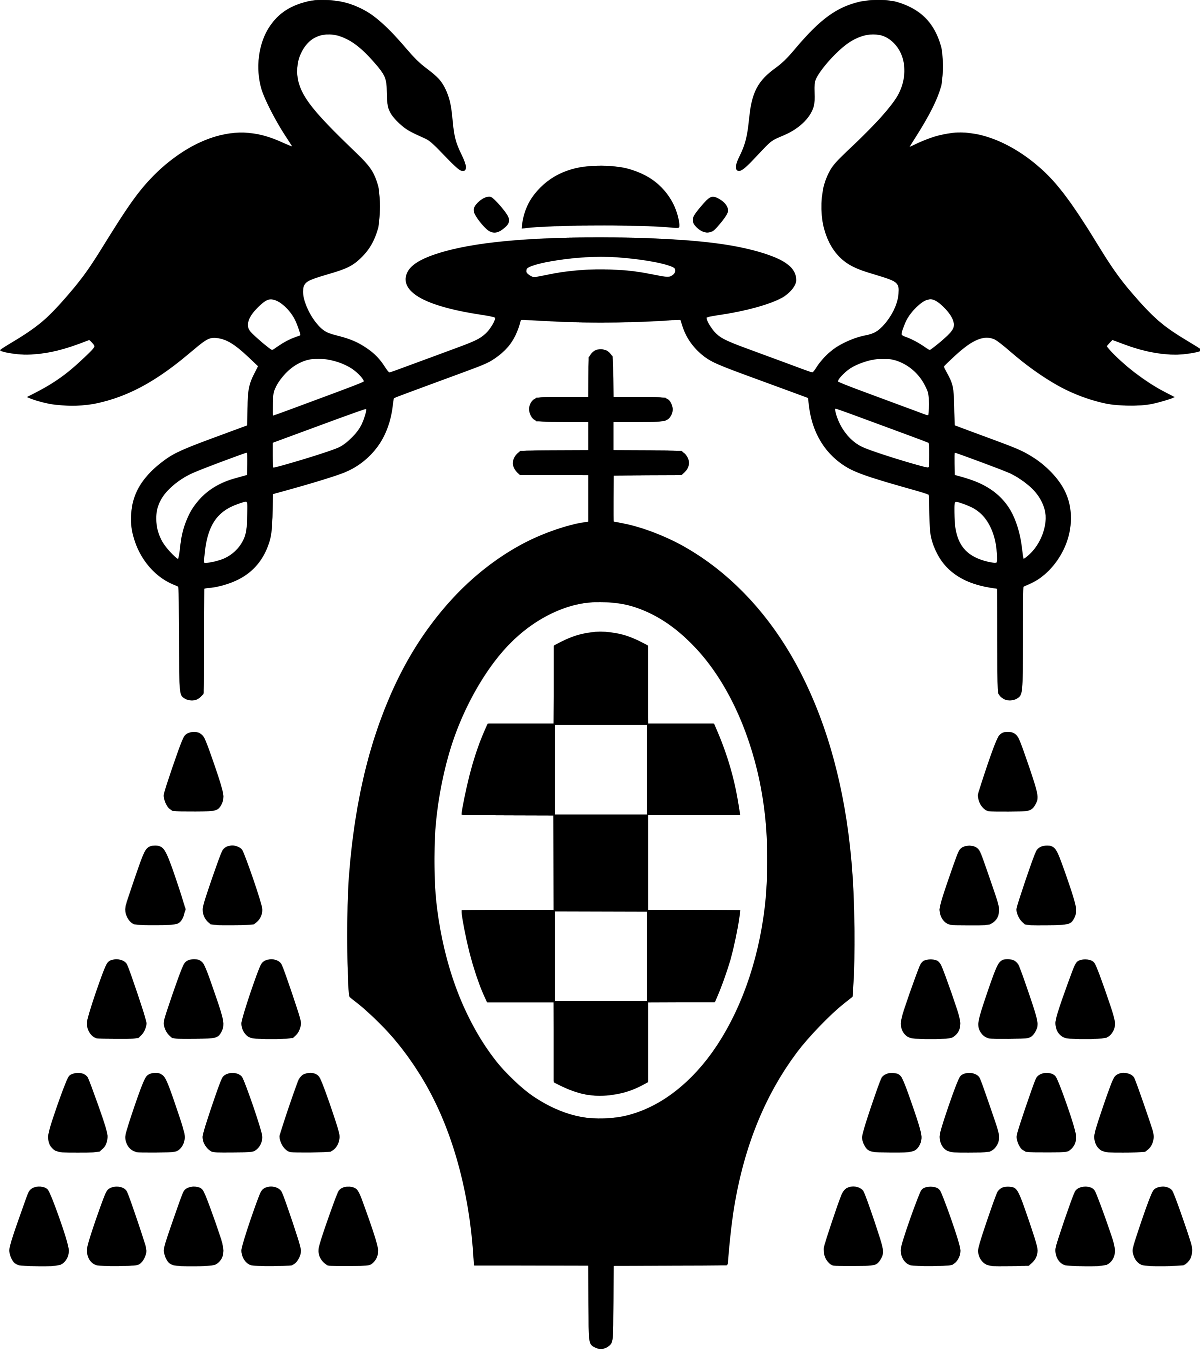
\includegraphics[scale = 0.075]{img/logo}
}

\author{
	Grupo 9\\\\
	Pablo García García\\
	Abel López Martínez\\
	Álvaro Jesús Martínez Parra\\
	Raúl Moratilla Núñez
}

\date{
	\large{\today}
}

\hypersetup{
	pdftitle = {Práctica 2}, 
	pdfauthor = {Pablo García García, Abel López Martínez, Álvaro Jesús Martínez Parra, Raúl Moratilla Núñez}, 
	pdfsubject = {Fundamentos de la Ciencia de Datos}, 
	pdfcenterwindow, 
	pdfnewwindow = true, 
	pdfkeywords = {Entrega de la PL2 de laboratorio correspondiente al Curso 2023-2024}, 
	bookmarksopen = true 
}

\newtheorem{exercise}{Ejercicio}[section]
\newtheorem{observation}{Observación}[section]
\newtcbtheorem[number within = section, Crefname = {Teorema}{Teorema}]{teorema}{Teorema}{fonttitle = \bfseries}{th}
\newtcbtheorem[number within = section, Crefname = {Definición}{Definición}]{definicion}{Definición}{fonttitle = \bfseries}{df}

\newcommand{\dt}{\text{dist}}
\newcommand{\ds}{\text{dens}}
\newcommand{\drm}{\text{drm}}

\newcommand{\rojo}[1]{\textcolor{Red}{#1}}
\IfFileExists{upquote.sty}{\usepackage{upquote}}{}
\begin{document}
	
	%Configuración para los gráficos de R
	
	
	\renewcommand{\chaptername}{Parte}
	\renewcommand{\lstlistingname}{Código}
	\maketitle \thispagestyle{empty}
	
	\newpage
	
	\setcounter{tocdepth}{3}
	\tableofcontents
	\listoffigures
	
	\chapter*{Introducción}\addcontentsline{toc}{chapter}{Introducción}\pagestyle{plain}
	
		\section*{RStudio}\addcontentsline{toc}{section}{RStudio}
	
			RStudio es un entorno de desarrollo integrado (IDE) para R, un lenguaje de programación ampliamente utilizado en estadística, análisis de datos, investigación científica y visualización de datos. Será empleado para el desarrollo de esta práctica. La interfaz del IDE de RStudio está diseñada para facilitar el análisis estadístico y la visualización de datos.
			
			\begin{itemize}
				
				\item \textbf{File}: Aquí puedes crear nuevos archivos y proyectos, incluidos scripts de Python y documentos Sweave. Trabajar con proyectos es una práctica profesional estándar y permite una mejor organización.
				
				\item \textbf{Edit}: Esta sección funciona de manera similar a otros entornos de desarrollo, proporcionando herramientas de edición de texto estándar.
				
				\item \textbf{Code}: Incluye herramientas específicas para escribir y ejecutar código R, como insertar operadores o ejecutar scripts completos.
				
				\item \textbf{View}: Permite ajustar la apariencia de la interfaz de RStudio, como mostrar u ocultar diferentes paneles.
				
				\item \textbf{Plots}: Muy utilizado para la visualización de datos, permite generar, ver y manipular gráficos estadísticos.
				
				\item \textbf{Session}: Controla las sesiones de R, permitiendo iniciar, interrumpir o terminar sesiones.
				
				\item \textbf{Build}: Herramientas relacionadas con la construcción de paquetes de R.
				
				\item \textbf{Debug}: Funciones para depurar el código R.
				
				\item \textbf{Profile}: Herramientas para medir el rendimiento del código R.
				
				\item \textbf{Tools}: Opciones para configurar el entorno de desarrollo globalmente, como la disposición del panel y opciones de proyecto.
				
				\item \textbf{Help}: Ofrece documentación y ayuda para usar R y RStudio, un recurso esencial para el aprendizaje y la solución de problemas.
				
			\end{itemize}
			
			El entorno de RStudio es altamente personalizable y se organiza en cuatro áreas principales. Puedes redactar código en el panel de \texttt{scripts}, ejecutar instrucciones en el \texttt{console}, y ver los objetos activos y el historial en el área de \texttt{environment/history}. El cuarto panel es multifuncional, permitiendo administrar archivos, visualizar datos a través de gráficos, instalar y administrar paquetes y buscar en la documentación en la sección indicada a continuación. 
			\begin{verbatim}
				files/plots/packages/help/viewer
			\end{verbatim}
			Este diseño modular facilita la gestión eficiente del flujo de trabajo en análisis de datos y desarrollo estadístico.
			
			\begin{figure}[H]
				\centering
				
\includegraphics[scale = 0.15]{img/rstudio}
				\caption{Logo del entorno RStudio}
				\label{fig:logo_rstudio}
			\end{figure}
			
		\section*{Posit}\addcontentsline{toc}{section}{Posit}
			
			La página web de Posit (\url{https://posit.co/}) ofrece una amplia gama de productos y soluciones para la ciencia de datos, enfocándose en el uso de R y Python. Presenta opciones de software de código abierto, soluciones empresariales y basadas en la nube. Destaca su compromiso con la ciencia de datos accesible para todos, ofreciendo recursos educativos, historias de clientes y soporte para la comunidad. La empresa busca promover un entorno inclusivo y empoderador, destacando su papel en el avance de la ciencia de datos a través de la colaboración y la innovación tecnológica.
				
			\begin{figure}[H]
				\centering
				
\includegraphics[scale = 0.15]{img/posit}
				\caption{Logo de la compañía Posit}
				\label{fig:logo_posit}
			\end{figure}
	
		\section*{De RStudio a Posit}\addcontentsline{toc}{section}{De RStudio a Posit}
	
			El artículo del blog de Posit (\url{https://posit.co/blog/rstudio-is-now-posit/}), anteriormente conocido como RStudio, detalla los cambios y compromisos de la compañía a medida que evoluciona. Fundada en 2009, RStudio se centró en crear software de código abierto de alta calidad para científicos de datos. La compañía ha invertido significativamente en el desarrollo de código abierto, educación y la comunidad, con el objetivo de servir a los creadores de conocimiento durante los próximos 100 años.\\
			
			La transformación de RStudio a Posit no solo implica un cambio de nombre, sino también una reafirmación de sus valores y objetivos. Como una Corporación de Beneficio Público y una B Corp certificada, Posit se compromete a cumplir con los más altos estándares de desempeño social y ambiental, transparencia y responsabilidad. Los directivos de Posit tienen la responsabilidad fiduciaria de abordar las necesidades sociales, económicas y ambientales, además de supervisar los objetivos comerciales de la empresa. La misión de Posit incluye mantener su independencia a largo plazo para cumplir con estos objetivos.\\
			
			El compromiso de Posit con el código abierto sigue siendo una prioridad central. La empresa cree firmemente que el progreso significativo se logra poniendo herramientas de ciencia de datos al alcance de todos, independientemente de sus medios económicos. Además, Posit busca expandir su enfoque más allá del lenguaje de programación R, abrazando también a la comunidad de Python y a otras comunidades de programación. Aunque R sigue siendo un componente clave, el objetivo es mejorar la comunicación científica para todos, creando software tanto de código abierto como comercial para R, Python y más.\\
			
			Finalmente, Posit desea fomentar una comunidad más amplia y diversa. Inspirándose en la comunidad de R, la compañía aspira a ayudar a que otras áreas de la ciencia sean tan abiertas, dinámicas, inclusivas y diversas como la comunidad a la que pertenecen. A pesar del cambio de nombre, la dedicación de Posit a ayudar a los científicos de datos a utilizar software de código abierto para plantear y responder preguntas importantes permanece inalterada.
	
	\chapter{Ejercicios guiados}\pagestyle{fancy}
	
		En esta primera parte de la práctica, se repetirán los ejercicios explicados y realizados por el profesor en las clases de laboratorio, utilizando los mismos procedimientos vistos y plasmándolos en este documento.
		
		\section{Clasificación no supervisada}
		
			\subsection{$k-$means}
		
				\begin{exercise}
					El primer conjunto de datos, que se empleará para realizar el análisis de clasificación no supervisada con $k-$means, estará formado por las siguientes 8 calificaciones de estudiantes: 1. \{4, 4\}; 2. \{3, 5\}; 3. \{1, 2\}; 4. \{5, 5\}; 5.\{0, 1\}; 6. \{2, 2\}; 7. \{4, 5\}; 8. \{2, 1\}, donde las características de las calificaciones son: \{Teoría, Laboratorio\}.
				\end{exercise}
				
				En este ejercicio se va a detallar cómo realizar una clasificación no supervisada en un conjunto de datos en R; concretamente utilizando el algoritmo $k-$means. El objetivo será agrupar subconjuntos de los datos en clústers o grupos, creando de esta forma una clasificación del conjunto total. Estos clústers se determinarán en base a la muestra, obteniéndose durante el mismo proceso de clasificación.\\
				
				El algoritmo $k-$means ofrece una técnica de clústerización en base a una muestra de datos y una cantidad $n$ de clústers. Para empezar a realizar el algoritmo se necesita la ubicación de los centroides de cada clúster. Un centroide es el punto medio del grupo de sucesos que componen el clúster, por lo que habrá tantos centroides como $n$ clústers haya. La cantidad de clústers así como sus centroides iniciales serán elegidos arbitrariamente por el usuario; estos se irán reubicando a medida que se itere en el algoritmo. \\
				
				Para empezar, en R se necesita introducir la muestra o conjunto de datos con el que se va a trabajar. Estos datos serán introducidos en una matriz utilizando la función \texttt{matrix}.
				
\begin{knitrout}
\definecolor{shadecolor}{rgb}{0.969, 0.969, 0.969}\color{fgcolor}\begin{kframe}
\begin{alltt}
\hlstd{m} \hlkwb{<-} \hlkwd{matrix}\hlstd{(}\hlkwd{c}\hlstd{(}\hlnum{4}\hlstd{,}\hlnum{4}\hlstd{,} \hlnum{3}\hlstd{,}\hlnum{5}\hlstd{,} \hlnum{1}\hlstd{,}\hlnum{2}\hlstd{,} \hlnum{5}\hlstd{,}\hlnum{5}\hlstd{,} \hlnum{0}\hlstd{,}\hlnum{1}\hlstd{,} \hlnum{2}\hlstd{,}\hlnum{2}\hlstd{,} \hlnum{4}\hlstd{,}\hlnum{5}\hlstd{,} \hlnum{2}\hlstd{,}\hlnum{1}\hlstd{),}\hlnum{2}\hlstd{,}\hlnum{8}\hlstd{)}
\hlstd{(m} \hlkwb{<-} \hlkwd{t}\hlstd{(m))}
\end{alltt}
\begin{verbatim}
##      [,1] [,2]
## [1,]    4    4
## [2,]    3    5
## [3,]    1    2
## [4,]    5    5
## [5,]    0    1
## [6,]    2    2
## [7,]    4    5
## [8,]    2    1
\end{verbatim}
\end{kframe}
\end{knitrout}
				
				Para poder trabajar debidamente se debe trasponer la matriz, de tal forma que cada columna represente una componente. El primer punto conformará la primera fila, el segundo punto la segunda fila y así sucesivamente con todos los datos.\\
				
				Además del conjunto de datos, el algoritmo $k-$means necesita unos centroides iniciales. Estos se introducirán de la misma forma que la muestra, teniendo en la primera fila el centroide del primer clúster, en la siguiente fila el centroide del segundo... Al tratarse de pocos puntos se eligen arbitrariamente dos centroides, por lo que la clasificación final será realizada con dos clústers. Se introducen así los centroides:
				
\begin{knitrout}
\definecolor{shadecolor}{rgb}{0.969, 0.969, 0.969}\color{fgcolor}\begin{kframe}
\begin{alltt}
\hlstd{c} \hlkwb{<-} \hlkwd{matrix}\hlstd{(}\hlkwd{c}\hlstd{(}\hlnum{0}\hlstd{,}\hlnum{1}\hlstd{,}\hlnum{2}\hlstd{,}\hlnum{2}\hlstd{),}\hlnum{2}\hlstd{,}\hlnum{2}\hlstd{)}
\hlstd{(c} \hlopt{< -}\hlkwd{t}\hlstd{(c))}
\end{alltt}
\begin{verbatim}
##       [,1]  [,2]
## [1,] FALSE FALSE
## [2,] FALSE FALSE
\end{verbatim}
\end{kframe}
\end{knitrout}
				
				Con la muestra y los centroides introducidos en el entorno de trabajo, ya se puede realizar el algoritmo. Para ello se utilizará la función \texttt{kmeans}, función del paquete cargado por defecto \texttt{stats}. La función recibe tres parámetros: la muestra de los datos (\texttt{m}), los centroides iniciales de los clústers (\texttt{c}) y el número de iteraciones que se desean. En este caso se eligen cuatro iteraciones, las mismas que se necesitaron en clase de teoría. En teoría, el número de iteraciones no se sabe a priori, por lo que habría que ir probando. Sin embargo, como ya se sabe el número que se necesita, se pone directamente 4.
				
				{\small
\begin{knitrout}
\definecolor{shadecolor}{rgb}{0.969, 0.969, 0.969}\color{fgcolor}\begin{kframe}
\begin{alltt}
\hlstd{(clasificacionns} \hlkwb{=} \hlstd{(}\hlkwd{kmeans}\hlstd{(m,c,}\hlnum{4}\hlstd{)))}
\end{alltt}
\begin{verbatim}
## K-means clustering with 2 clusters of sizes 4, 4
## 
## Cluster means:
##   [,1] [,2]
## 1 1.25 1.50
## 2 4.00 4.75
## 
## Clustering vector:
## [1] 2 2 1 2 1 1 2 1
## 
## Within cluster sum of squares by cluster:
## [1] 3.75 2.75
##  (between_SS / total_SS =  84.8 %)
## 
## Available components:
## 
## [1] "cluster"      "centers"      "totss"        "withinss"     "tot.withinss"
## [6] "betweenss"    "size"         "iter"         "ifault"
\end{verbatim}
\end{kframe}
\end{knitrout}
				}
				
				Entre los parámetros que aparecen en la salida se encuentran \texttt{Cluster means} y \texttt{Clustering vector}. El primero de ellos proporciona la ubicación de los dos centroides de los clústers que conforman la clasificación final. Como se puede apreciar, salen los dos centroides que salieron en teoría. El segundo parámetro indica a qué clúster pertenece cada suceso de la muestra introducida. Así el punto 1 pertenece al clúster 2, el punto 2 pertenece al clúster 2, el punto 3 al clúster 1... Este último se puede utilizar como entrada para realizar otras tareas. Puede ser muy útil para analizar cada clúster por separado, ver sus caracteristicas comunes e intentar deducir por qué esos datos están relacionados.\\
				
				El siguiente comando permite añadir una columna a la izquierda de la muestra de datos (\texttt{m}) que se había introducido al inicio, indicando a qué clúster pertenece cada suceso.
				
\begin{knitrout}
\definecolor{shadecolor}{rgb}{0.969, 0.969, 0.969}\color{fgcolor}\begin{kframe}
\begin{alltt}
\hlstd{(m} \hlkwb{=} \hlkwd{cbind}\hlstd{(clasificacionns}\hlopt{$}\hlstd{clúster,m))}
\end{alltt}
\begin{verbatim}
##      [,1] [,2]
## [1,]    4    4
## [2,]    3    5
## [3,]    1    2
## [4,]    5    5
## [5,]    0    1
## [6,]    2    2
## [7,]    4    5
## [8,]    2    1
\end{verbatim}
\end{kframe}
\end{knitrout}
				
				Esto se realiza para poder dividir la muestra según la clasificación que se ha conseguido. Llamando a la función subset se puede extraer la porción de la muestra que pertenece al clúster 1 y la porción restante que pertenece al clúster 2.
				
\begin{knitrout}
\definecolor{shadecolor}{rgb}{0.969, 0.969, 0.969}\color{fgcolor}\begin{kframe}
\begin{alltt}
\hlstd{(mc1} \hlkwb{=} \hlkwd{subset}\hlstd{(m,m[,}\hlnum{1}\hlstd{]}\hlopt{==}\hlnum{1}\hlstd{))}
\end{alltt}
\begin{verbatim}
##      [,1] [,2]
## [1,]    1    2
\end{verbatim}
\begin{alltt}
\hlstd{(mc2} \hlkwb{=} \hlkwd{subset}\hlstd{(m,m[,}\hlnum{1}\hlstd{]}\hlopt{==}\hlnum{2}\hlstd{))}
\end{alltt}
\begin{verbatim}
##      [,1] [,2]
## [1,]    2    2
## [2,]    2    1
\end{verbatim}
\end{kframe}
\end{knitrout}
				
				Una vez se tienen los datos separados se puede eliminar la columna que indica el clúster al que pertenece cada dato, ya que se sobreentiende que todos pertenecen al mismo clúster porque ya han pasado por un proceso de separación en función de la clasificación. Por ejemplo, para los datos pertenecientes al primer clúster, se haría de la siguiente forma:
				
\begin{knitrout}
\definecolor{shadecolor}{rgb}{0.969, 0.969, 0.969}\color{fgcolor}\begin{kframe}
\begin{alltt}
\hlstd{(mc1} \hlkwb{=} \hlstd{mc1[,}\hlopt{-}\hlnum{1}\hlstd{])}
\end{alltt}
\begin{verbatim}
## [1] 2
\end{verbatim}
\end{kframe}
\end{knitrout}
				
				Con todo esto se consigue, partiendo de una muestra de datos, una clasificación no supervisada utilizando la técnica de clústerización basada en el algoritmo $k-$means. A partir de ella se podrán intentar deducir ciertas conclusiones.
		
			\subsection{Clusterización jerárquica algomerativa}
		
				\begin{exercise}
					El segundo conjunto de datos, que se empleará para realizar el análisis de clasificación no supervisada con Clusterización Jerárquica Aglomerativa, estará formado por 6 calificaciones de estudiantes: 1. \{0.89, 2.94\}; 2.\{4.36, 5.21\}; 3. \{3.75, 1.12\}; 4. \{6.25, 3.14\}; 5. \{4.1, 1.8\}; 6. \{3.9, 4.27\}.
				\end{exercise}
				
				La Clusterización Jerárquica Aglomerativa es un método de análisis de datos que comienza tratando cada punto como un clúster individual y luego, iterativamente, combina los clústers más cercanos hasta formar un único clúster. Este método es útil para identificar grupos naturales en los datos. En clase se implementó mediante el paquete \texttt{LearnClust} del CRAN.\\
				
				Inicialmente, se crea una matriz con la muestra del problema, y se transpone la matriz para que tenga el formato deseado.
				
\begin{knitrout}
\definecolor{shadecolor}{rgb}{0.969, 0.969, 0.969}\color{fgcolor}\begin{kframe}
\begin{alltt}
\hlstd{m} \hlkwb{<-} \hlkwd{matrix}\hlstd{(}
        \hlkwd{c}\hlstd{(}\hlnum{0.89}\hlstd{,}\hlnum{2.94}\hlstd{,} \hlnum{4.36}\hlstd{,}\hlnum{5.21}\hlstd{,} \hlnum{3.75}\hlstd{,}\hlnum{1.12}\hlstd{,} \hlnum{6.25}\hlstd{,}\hlnum{3.14}\hlstd{,} \hlnum{4.1}\hlstd{,}\hlnum{1.8}\hlstd{,} \hlnum{3.9}\hlstd{,}\hlnum{4.27}\hlstd{),}\hlnum{2}\hlstd{,}\hlnum{6}\hlstd{)}
\hlstd{(m} \hlkwb{<-} \hlkwd{t}\hlstd{(m))}
\end{alltt}
\begin{verbatim}
##      [,1] [,2]
## [1,] 0.89 2.94
## [2,] 4.36 5.21
## [3,] 3.75 1.12
## [4,] 6.25 3.14
## [5,] 4.10 1.80
## [6,] 3.90 4.27
\end{verbatim}
\end{kframe}
\end{knitrout}
				
				Para la ejecución del algoritmo utilizamos la función \texttt{agglomerativeHC}. Esta función recibe como parámetros la matriz de datos, la métrica de distancia y el criterio de enlace.
				
\begin{knitrout}
\definecolor{shadecolor}{rgb}{0.969, 0.969, 0.969}\color{fgcolor}\begin{kframe}
\begin{alltt}
\hlkwd{agglomerativeHC}\hlstd{(m,} \hlstr{'EUC'}\hlstd{,} \hlstr{'MIN'}\hlstd{)}
\end{alltt}
\begin{verbatim}
## $dendrogram
## Number of objects: 6 
## 
## 
## $clusters
## $clusters[[1]]
##     X1   X2
## 1 0.89 2.94
## 
## $clusters[[2]]
##     X1   X2
## 1 4.36 5.21
## 
## $clusters[[3]]
##     X1   X2
## 1 3.75 1.12
## 
## $clusters[[4]]
##     X1   X2
## 1 6.25 3.14
## 
## $clusters[[5]]
##    X1  X2
## 1 4.1 1.8
## 
## $clusters[[6]]
##    X1   X2
## 1 3.9 4.27
## 
## $clusters[[7]]
##     X1   X2
## 1 3.75 1.12
## 2 4.10 1.80
## 
## $clusters[[8]]
##     X1   X2
## 1 4.36 5.21
## 2 3.90 4.27
## 
## $clusters[[9]]
##     X1   X2
## 1 3.75 1.12
## 2 4.10 1.80
## 3 4.36 5.21
## 4 3.90 4.27
## 
## $clusters[[10]]
##     X1   X2
## 1 6.25 3.14
## 2 3.75 1.12
## 3 4.10 1.80
## 4 4.36 5.21
## 5 3.90 4.27
## 
## $clusters[[11]]
##     X1   X2
## 1 0.89 2.94
## 2 6.25 3.14
## 3 3.75 1.12
## 4 4.10 1.80
## 5 4.36 5.21
## 6 3.90 4.27
## 
## 
## $groupedClusters
##   cluster1 cluster2
## 1        3        5
## 2        2        6
## 3        7        8
## 4        4        9
## 5        1       10
\end{verbatim}
\end{kframe}
\end{knitrout}
				
				En este código, \texttt{EUC} representa la métrica de distancia euclidiana y \texttt{MIN} el criterio para la agrupación de clústers. En la salida se pueden observar cuatro apartados.
				
				\begin{itemize}
					\item El primero es una figura los datos de la matriz que hemos introducido impresos en una gráfica.
					
					\item El segundo es el número de puntos que se han introducido, mediante el atributo \texttt{\$dendrogram}, en este caso 6.
					
					\item El tercer apartado es una lista que muestra las coordenadas de todos los clústers al finalizar la ejecución, los 6 primeros son los puntos introducidos y los 5 siguientes son los formados por cada una de las iteraciones uniendo dos clústers anteriores hasta tener todos unidos en el mismo clúster, momento en el que finaliza el algoritmo. Se puede ver en el atributo \texttt{\$clústers}.
					
					\item El cuarto apartado es el proceso que se realiza en cada iteración, se pueden ver en el apartado \texttt{\$groupedClusters}.
					
					\begin{enumerate}[label = \textbf{\arabic*.}]
						\item Se unen los clústers 3 y 5, para formar el clúster 7.
						\item Se unen los clústers 2 y 6, para formar el clúster 8.
						\item Se unen los clústers 4 y 8, para formar el clúster 9.
						\item Se unen los clústers 7 y 9, para formar el clúster 10.
						\item Se unen los clústers 1 y 10, para formar el clúster 11.
					\end{enumerate}
					
				\end{itemize}
				
				Para obtener una explicación detallada paso a paso tal y como se ha explicado en clase, usamos la función \texttt{agglomerativeHC.details}.
				
				{
				\footnotesize
\begin{knitrout}
\definecolor{shadecolor}{rgb}{0.969, 0.969, 0.969}\color{fgcolor}\begin{kframe}
\begin{alltt}
\hlkwd{agglomerativeHC.details}\hlstd{(m,} \hlstr{'EUC'}\hlstd{,} \hlstr{'MIN'}\hlstd{)}
\end{alltt}


{\ttfamily\noindent\itshape\color{messagecolor}{\#\# \ \ Agglomerative hierarchical clustering is a classification technique that initializes \\\#\# \ a cluster for each data.}}

{\ttfamily\noindent\itshape\color{messagecolor}{\#\# \\\#\# \ \ It calculates the distance between datas depending on the approach type given and}}

{\ttfamily\noindent\itshape\color{messagecolor}{\#\# \\\#\# \ it creates a new cluster joining the most similar clusters until getting only one.}}

{\ttfamily\noindent\itshape\color{messagecolor}{\#\# \ \ 'toList' creates a list initializing datas by creating clusters with each one}}

{\ttfamily\noindent\itshape\color{messagecolor}{\#\# \\\#\# \ \ These are the clusters with only one element:}}\begin{verbatim}
## [[1]]
##      [,1] [,2] [,3]
## [1,] 0.89 2.94    1
## 
## [[2]]
##      [,1] [,2] [,3]
## [1,] 4.36 5.21    1
## 
## [[3]]
##      [,1] [,2] [,3]
## [1,] 3.75 1.12    1
## 
## [[4]]
##      [,1] [,2] [,3]
## [1,] 6.25 3.14    1
## 
## [[5]]
##      [,1] [,2] [,3]
## [1,]  4.1  1.8    1
## 
## [[6]]
##      [,1] [,2] [,3]
## [1,]  3.9 4.27    1
\end{verbatim}


{\ttfamily\noindent\itshape\color{messagecolor}{\#\# \\\#\# \ \ In each step: \\\#\# \ \ \ - It calculates a matrix distance between active clusters depending on the approach and distance type.}}

{\ttfamily\noindent\itshape\color{messagecolor}{\#\# \ \ \ - It gets the minimum distance value from the matrix.}}

{\ttfamily\noindent\itshape\color{messagecolor}{\#\# \ \ \ - It creates a new cluster joining the minimum distance clusters.}}

{\ttfamily\noindent\itshape\color{messagecolor}{\#\# \ \ \ - It repeats these steps while final clusters do not include all datas.}}

{\ttfamily\noindent\itshape\color{messagecolor}{\#\# \\\#\# \_\_\_\_\_\_\_\_\_\_\_\_\_\_\_\_\_\_\_\_\_\_\_\_\_\_\_\_\_\_\_\_\_\_\_\_\_\_\_\_\_\_\_\_\_\_\_\_\_\_\_\_\_\_\_\_\_\_\_\_\_\_\_\_\_\_\_\_\_\_\_\_\_\_\_\_\_\_\_\_\_\_\_\_\_\_\_\_\_\_\_\_\_}}

{\ttfamily\noindent\itshape\color{messagecolor}{\#\# STEP => 1}}

{\ttfamily\noindent\itshape\color{messagecolor}{\#\# \\\#\# \ Matrix Distance (distance type = EUC, approach type = MIN):}}\begin{verbatim}
##          [,1]     [,2]      [,3]     [,4]      [,5]     [,6]
## [1,] 0.000000 4.146541 3.3899853 5.363730 3.4064204 3.290745
## [2,] 4.146541 0.000000 4.1352388 2.803034 3.4198977 1.046518
## [3,] 3.389985 4.135239 0.0000000 3.214094 0.7647876 3.153569
## [4,] 5.363730 2.803034 3.2140940 0.000000 2.5333969 2.607566
## [5,] 3.406420 3.419898 0.7647876 2.533397 0.0000000 2.478084
## [6,] 3.290745 1.046518 3.1535694 2.607566 2.4780839 0.000000
\end{verbatim}


{\ttfamily\noindent\itshape\color{messagecolor}{\#\# \\\#\# \ The minimum distance is: 0.764787552199956}}

{\ttfamily\noindent\itshape\color{messagecolor}{\#\# \\\#\# \ The closest clusters are: 3, 5}}

{\ttfamily\noindent\itshape\color{messagecolor}{\#\# \\\#\# \ The grouped clusters are added to the solution.}}

{\ttfamily\noindent\itshape\color{messagecolor}{\#\# \\\#\# \ Grouping clusters 3 and cluster 5, it is created a new cluster:}}\begin{verbatim}
##     X1   X2
## 1 3.75 1.12
## 2 4.10 1.80
\end{verbatim}


{\ttfamily\noindent\itshape\color{messagecolor}{\#\# \\\#\# \ The new cluster is added to the solution.}}

{\ttfamily\noindent\itshape\color{messagecolor}{\#\# \\\#\# \_\_\_\_\_\_\_\_\_\_\_\_\_\_\_\_\_\_\_\_\_\_\_\_\_\_\_\_\_\_\_\_\_\_\_\_\_\_\_\_\_\_\_\_\_\_\_\_\_\_\_\_\_\_\_\_\_\_\_\_\_\_\_\_\_\_\_\_\_\_\_\_\_\_\_\_\_\_\_\_\_\_\_\_\_\_\_\_\_\_\_\_\_}}

{\ttfamily\noindent\itshape\color{messagecolor}{\#\# STEP => 2}}

{\ttfamily\noindent\itshape\color{messagecolor}{\#\# \\\#\# \ Matrix Distance (distance type = EUC, approach type = MIN):}}\begin{verbatim}
##          [,1]     [,2] [,3]     [,4] [,5]     [,6]     [,7]
## [1,] 0.000000 4.146541    0 5.363730    0 3.290745 3.389985
## [2,] 4.146541 0.000000    0 2.803034    0 1.046518 3.419898
## [3,] 0.000000 0.000000    0 0.000000    0 0.000000 0.000000
## [4,] 5.363730 2.803034    0 0.000000    0 2.607566 2.533397
## [5,] 0.000000 0.000000    0 0.000000    0 0.000000 0.000000
## [6,] 3.290745 1.046518    0 2.607566    0 0.000000 2.478084
## [7,] 3.389985 3.419898    0 2.533397    0 2.478084 0.000000
\end{verbatim}


{\ttfamily\noindent\itshape\color{messagecolor}{\#\# \\\#\# \ The minimum distance is: 1.04651803615609}}

{\ttfamily\noindent\itshape\color{messagecolor}{\#\# \\\#\# \ The closest clusters are: 2, 6}}

{\ttfamily\noindent\itshape\color{messagecolor}{\#\# \\\#\# \ The grouped clusters are added to the solution.}}

{\ttfamily\noindent\itshape\color{messagecolor}{\#\# \\\#\# \ Grouping clusters 2 and cluster 6, it is created a new cluster:}}\begin{verbatim}
##     X1   X2
## 1 4.36 5.21
## 2 3.90 4.27
\end{verbatim}


{\ttfamily\noindent\itshape\color{messagecolor}{\#\# \\\#\# \ The new cluster is added to the solution.}}

{\ttfamily\noindent\itshape\color{messagecolor}{\#\# \\\#\# \_\_\_\_\_\_\_\_\_\_\_\_\_\_\_\_\_\_\_\_\_\_\_\_\_\_\_\_\_\_\_\_\_\_\_\_\_\_\_\_\_\_\_\_\_\_\_\_\_\_\_\_\_\_\_\_\_\_\_\_\_\_\_\_\_\_\_\_\_\_\_\_\_\_\_\_\_\_\_\_\_\_\_\_\_\_\_\_\_\_\_\_\_}}

{\ttfamily\noindent\itshape\color{messagecolor}{\#\# STEP => 3}}

{\ttfamily\noindent\itshape\color{messagecolor}{\#\# \\\#\# \ Matrix Distance (distance type = EUC, approach type = MIN):}}\begin{verbatim}
##          [,1] [,2] [,3]     [,4] [,5] [,6]     [,7]     [,8]
## [1,] 0.000000    0    0 5.363730    0    0 3.389985 3.290745
## [2,] 0.000000    0    0 0.000000    0    0 0.000000 0.000000
## [3,] 0.000000    0    0 0.000000    0    0 0.000000 0.000000
## [4,] 5.363730    0    0 0.000000    0    0 2.533397 2.607566
## [5,] 0.000000    0    0 0.000000    0    0 0.000000 0.000000
## [6,] 0.000000    0    0 0.000000    0    0 0.000000 0.000000
## [7,] 3.389985    0    0 2.533397    0    0 0.000000 2.478084
## [8,] 3.290745    0    0 2.607566    0    0 2.478084 0.000000
\end{verbatim}


{\ttfamily\noindent\itshape\color{messagecolor}{\#\# \\\#\# \ The minimum distance is: 2.47808393723861}}

{\ttfamily\noindent\itshape\color{messagecolor}{\#\# \\\#\# \ The closest clusters are: 7, 8}}

{\ttfamily\noindent\itshape\color{messagecolor}{\#\# \\\#\# \ The grouped clusters are added to the solution.}}

{\ttfamily\noindent\itshape\color{messagecolor}{\#\# \\\#\# \ Grouping clusters 7 and cluster 8, it is created a new cluster:}}\begin{verbatim}
##     X1   X2
## 1 3.75 1.12
## 2 4.10 1.80
## 3 4.36 5.21
## 4 3.90 4.27
\end{verbatim}


{\ttfamily\noindent\itshape\color{messagecolor}{\#\# \\\#\# \ The new cluster is added to the solution.}}

{\ttfamily\noindent\itshape\color{messagecolor}{\#\# \\\#\# \_\_\_\_\_\_\_\_\_\_\_\_\_\_\_\_\_\_\_\_\_\_\_\_\_\_\_\_\_\_\_\_\_\_\_\_\_\_\_\_\_\_\_\_\_\_\_\_\_\_\_\_\_\_\_\_\_\_\_\_\_\_\_\_\_\_\_\_\_\_\_\_\_\_\_\_\_\_\_\_\_\_\_\_\_\_\_\_\_\_\_\_\_}}

{\ttfamily\noindent\itshape\color{messagecolor}{\#\# STEP => 4}}

{\ttfamily\noindent\itshape\color{messagecolor}{\#\# \\\#\# \ Matrix Distance (distance type = EUC, approach type = MIN):}}\begin{verbatim}
##           [,1] [,2] [,3]     [,4] [,5] [,6] [,7] [,8]     [,9]
##  [1,] 0.000000    0    0 5.363730    0    0    0    0 3.290745
##  [2,] 0.000000    0    0 0.000000    0    0    0    0 0.000000
##  [3,] 0.000000    0    0 0.000000    0    0    0    0 0.000000
##  [4,] 5.363730    0    0 0.000000    0    0    0    0 2.533397
##  [5,] 0.000000    0    0 0.000000    0    0    0    0 0.000000
##  [6,] 0.000000    0    0 0.000000    0    0    0    0 0.000000
##  [7,] 0.000000    0    0 0.000000    0    0    0    0 0.000000
##  [8,] 0.000000    0    0 0.000000    0    0    0    0 0.000000
##  [9,] 3.290745    0    0 2.533397    0    0    0    0 0.000000
\end{verbatim}


{\ttfamily\noindent\itshape\color{messagecolor}{\#\# \\\#\# \ The minimum distance is: 2.53339692902632}}

{\ttfamily\noindent\itshape\color{messagecolor}{\#\# \\\#\# \ The closest clusters are: 4, 9}}

{\ttfamily\noindent\itshape\color{messagecolor}{\#\# \\\#\# \ The grouped clusters are added to the solution.}}

{\ttfamily\noindent\itshape\color{messagecolor}{\#\# \\\#\# \ Grouping clusters 4 and cluster 9, it is created a new cluster:}}\begin{verbatim}
##     X1   X2
## 1 6.25 3.14
## 2 3.75 1.12
## 3 4.10 1.80
## 4 4.36 5.21
## 5 3.90 4.27
\end{verbatim}


{\ttfamily\noindent\itshape\color{messagecolor}{\#\# \\\#\# \ The new cluster is added to the solution.}}

{\ttfamily\noindent\itshape\color{messagecolor}{\#\# \\\#\# \_\_\_\_\_\_\_\_\_\_\_\_\_\_\_\_\_\_\_\_\_\_\_\_\_\_\_\_\_\_\_\_\_\_\_\_\_\_\_\_\_\_\_\_\_\_\_\_\_\_\_\_\_\_\_\_\_\_\_\_\_\_\_\_\_\_\_\_\_\_\_\_\_\_\_\_\_\_\_\_\_\_\_\_\_\_\_\_\_\_\_\_\_}}

{\ttfamily\noindent\itshape\color{messagecolor}{\#\# STEP => 5}}

{\ttfamily\noindent\itshape\color{messagecolor}{\#\# \\\#\# \ Matrix Distance (distance type = EUC, approach type = MIN):}}\begin{verbatim}
##           [,1] [,2] [,3] [,4] [,5] [,6] [,7] [,8] [,9]    [,10]
##  [1,] 0.000000    0    0    0    0    0    0    0    0 3.290745
##  [2,] 0.000000    0    0    0    0    0    0    0    0 0.000000
##  [3,] 0.000000    0    0    0    0    0    0    0    0 0.000000
##  [4,] 0.000000    0    0    0    0    0    0    0    0 0.000000
##  [5,] 0.000000    0    0    0    0    0    0    0    0 0.000000
##  [6,] 0.000000    0    0    0    0    0    0    0    0 0.000000
##  [7,] 0.000000    0    0    0    0    0    0    0    0 0.000000
##  [8,] 0.000000    0    0    0    0    0    0    0    0 0.000000
##  [9,] 0.000000    0    0    0    0    0    0    0    0 0.000000
## [10,] 3.290745    0    0    0    0    0    0    0    0 0.000000
\end{verbatim}


{\ttfamily\noindent\itshape\color{messagecolor}{\#\# \\\#\# \ The minimum distance is: 3.29074459659208}}

{\ttfamily\noindent\itshape\color{messagecolor}{\#\# \\\#\# \ The closest clusters are: 1, 10}}

{\ttfamily\noindent\itshape\color{messagecolor}{\#\# \\\#\# \ The grouped clusters are added to the solution.}}

{\ttfamily\noindent\itshape\color{messagecolor}{\#\# \\\#\# \ Grouping clusters 1 and cluster 10, it is created a new cluster:}}\begin{verbatim}
##     X1   X2
## 1 0.89 2.94
## 2 6.25 3.14
## 3 3.75 1.12
## 4 4.10 1.80
## 5 4.36 5.21
## 6 3.90 4.27
\end{verbatim}


{\ttfamily\noindent\itshape\color{messagecolor}{\#\# \\\#\# \ The new cluster is added to the solution.}}

{\ttfamily\noindent\itshape\color{messagecolor}{\#\# \\\#\# \ This loop has been repeated until the last cluster contained every single clusters.}}\end{kframe}\begin{figure}

{\centering 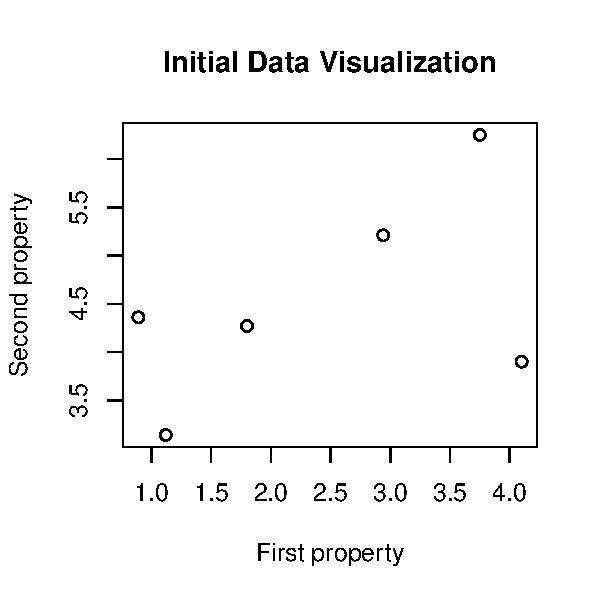
\includegraphics[width=\maxwidth]{figure/unnamed-chunk-9-1} 

}

\caption[Diagrama de LearnClust]{Diagrama de LearnClust}\label{fig:unnamed-chunk-9}
\end{figure}

\end{knitrout}
				}
				
				La función también se puede ejecutar con diferentes criterios de unión, como \texttt{MAX} y \texttt{AVG}, para observar cómo cambian los clústers:
				
				\begin{verbatim}
					agglomerativeHC.details(m, 'EUC', 'MAX')
					agglomerativeHC.details(m, 'EUC', 'AVG')
				\end{verbatim}
		
		\section{Clasificación supervisada}
		
			\subsection{Árboles de decisión}
		
				\begin{exercise}
					El tercer conjunto de datos, que se empleará para realizar el análisis de clasificación supervisada utilizando árboles de decisión, estará formado por las siguientes 9 calificaciones de estudiantes: 1. \{A, A, B, Ap\}; 2. \{A, B, D, Ss\}; 3. \{D, D, C, Ss\}; 4. \{D, D, A, Ss\}; 5. \{B, C, B, Ss\}; 6. \{C, B, B, Ap\}; 7. \{B, B, A, Ap\}; 8. \{C, D, C, Ss\}; 9. \{B, A, C,
					Ss\}, donde las características de las calificaciones son: \{Teoría, Laboratorio, Prácticas, Calificación Global).
				\end{exercise}
				
				El primer paso a ejecutar para poder realizar la clasificación supervisada con árboles de decisión es introducir los datos en un archivo de texto (\texttt{.txt}), que será posteriormente leído con el lenguaje R. Para ello, es necesario que el archivo de texto cumpla con un formato en concreto:
				
				\begin{itemize}
					\item La primera fila contendrá los nombres de las columnas, iniciando la fila con un tabulado o espacio e introduciendo otro entre cada una de las columnas.
					\item La primera columna contendrá los nombres de cada una de las filas del dataframe.
					\item Cada elemento de una fila estará separado del resto con un tabulado o espacio.
					\item El archivo de texto debe finalizar con una fila vacía.
				\end{itemize}
				
				Este archivo de texto se llamará \texttt{aprobados.txt} y será guardado en la carpeta \texttt{data}. El archivo es cargado en R de la siguiente forma:
				
\begin{knitrout}
\definecolor{shadecolor}{rgb}{0.969, 0.969, 0.969}\color{fgcolor}\begin{kframe}
\begin{alltt}
\hlstd{(calificaciones}\hlkwb{=}\hlkwd{read.table}\hlstd{(}\hlstr{"data/aprobados.txt"}\hlstd{))}
\end{alltt}
\begin{verbatim}
##    T L P CG
## 1. A A B Ap
## 2. A B D Ss
## 3. D D C Ss
## 4. D D A Ss
## 5. B C B Ss
## 6. C B B Ap
## 7. B B A Ap
## 8. C D C Ss
## 9. B A C Ss
\end{verbatim}
\end{kframe}
\end{knitrout}
				
				Para la implementación del algoritmo, se emplea el paquete \texttt{rpart}, el cual se encuentra disponible en el repositorio \texttt{CRAN}. Este paquete ofrece un método homónimo que recibe por parámetro, entre otros, los datos en forma de dataframe. Por ello, es necesario poseer los datos en esta forma en lugar de en una tabla:
				
\begin{knitrout}
\definecolor{shadecolor}{rgb}{0.969, 0.969, 0.969}\color{fgcolor}\begin{kframe}
\begin{alltt}
\hlstd{(muestra}\hlkwb{=}\hlkwd{data.frame}\hlstd{(calificaciones))}
\end{alltt}
\begin{verbatim}
##    T L P CG
## 1. A A B Ap
## 2. A B D Ss
## 3. D D C Ss
## 4. D D A Ss
## 5. B C B Ss
## 6. C B B Ap
## 7. B B A Ap
## 8. C D C Ss
## 9. B A C Ss
\end{verbatim}
\begin{alltt}
\hlstd{clasificacion} \hlkwb{=} \hlkwd{rpart}\hlstd{(CG}\hlopt{~}\hlstd{T}\hlopt{+}\hlstd{L}\hlopt{+}\hlstd{P,} \hlkwc{data}\hlstd{=muestra,} \hlkwc{method}\hlstd{=}\hlstr{"class"}\hlstd{,} \hlkwc{minsplit}\hlstd{=}\hlnum{1}\hlstd{)}
\end{alltt}
\end{kframe}
\end{knitrout}
				
				El primer argumento que se le pasa es \texttt{CG~T+L+P}, que contiene como primer elemento (a la izquierda de \texttt{\~}) el criterio que se desea clasificar, y a la derecha de la virgulilla, aparecen las columnas sobre las que se desea clasificar. También es posible poner un punto (\texttt{.}) a la derecha, lo cual significa que se clasificaría en base a todas las columnas que no fueran el criterio de clasificación. El segundo parámetro es, como ya se ha mencionado, la muestra en un dataframe; el tercer parámetro \texttt{ method='class'} indica que se está abordando un problema de clasificación; y el último parámetro \texttt{minsplit=1} es necesario ya que se está trabajando sobre un conjunto de datos pequeño. La salida de la función es la siguiente:
				
\begin{knitrout}
\definecolor{shadecolor}{rgb}{0.969, 0.969, 0.969}\color{fgcolor}\begin{kframe}
\begin{alltt}
\hlstd{clasificacion}
\end{alltt}
\begin{verbatim}
## n= 9 
## 
## node), split, n, loss, yval, (yprob)
##       * denotes terminal node
## 
## 1) root 9 3 Ss (0.3333333 0.6666667)  
##   2) L=A,B 5 2 Ap (0.6000000 0.4000000)  
##     4) P=A,B 3 0 Ap (1.0000000 0.0000000) *
##     5) P=C,D 2 0 Ss (0.0000000 1.0000000) *
##   3) L=C,D 4 0 Ss (0.0000000 1.0000000) *
\end{verbatim}
\end{kframe}
\end{knitrout}
				
				Se puede apreciar que el árbol consta de dos niveles además de la raíz. El primero de ellos clasifica según la nota en laboratorio. En caso de ser \texttt{C} o \texttt{D}, la calificación final es \texttt{Ss}, en caso de ser \texttt{A} o \texttt{B} es necesario observar el siguiente nivel. Este segundo nivel clasifica según la nota de prácticas, si la nota es \texttt{A} o \texttt{B}, la calificación es \texttt{Ap} y si es \texttt{C} o \texttt{D}, la calificación final es \texttt{Ss}.
		
		\subsection{Regresión lineal}
		
			\begin{exercise}
				El cuarto conjunto de datos, que se empleará para realizar el análisis de clasificación supervisada utilizando regresión, estará formado por los siguientes 4 radios ecuatoriales y densidades de los planetas interiores:
				\{Mercurio, 2.4, 5.4; Venus, 6.1, 5.2; Tierra, 6.4, 5.5; Marte, 3.4, 3.9\}.
			\end{exercise}
			
			Para empezar este ejercicio se deberán introducir los datos expuestos en el enunciado en un archivo de texto (\texttt{.txt}), con el fin de ser posteriormente leídos. La inserción de los datos en este fichero se hará atendiendo a las normas relacionadas con este tipo de archivos que ya se vieron en la primera práctica. Estas normas son las siguientes:
			
			\begin{itemize}
				\item Existirá una tabulación entre dato y dato. 
				\item La primera columna numera las filas, y en la primera fila se introduce un espacio y el nombre de las variables. 
				\item Se introducirá un salto de línea en la última fila. 
				\item Para los números decimales se utilizarán puntos. 
				\item Al escribir nombres, no se deberán introducir espacios. 
			\end{itemize}
			
			Obedeciendo estas normas, se copian los datos en un fichero llamado \texttt{planetas.txt}, y se carga en R de la siguiente manera:
			
\begin{knitrout}
\definecolor{shadecolor}{rgb}{0.969, 0.969, 0.969}\color{fgcolor}\begin{kframe}
\begin{alltt}
\hlstd{(muestra} \hlkwb{=} \hlkwd{read.table}\hlstd{(}\hlstr{"data/planetas.txt"}\hlstd{))}
\end{alltt}
\begin{verbatim}
##      R   D
## 1. 2.4 5.4
## 2. 6.1 5.2
## 3. 6.4 5.5
## 4. 3.4 3.9
\end{verbatim}
\end{kframe}
\end{knitrout}
			
			Una vez se tienen los datos en R, se procede a hacer uso de la función \texttt{lm} contenida en los paquetes básicos (concretamente en el paquete \texttt{stats}). Esta función recibe dos parámetros. El primero de ellos es la fórmula en donde se va a decir en función de qué parámetro se quiere otro parámetro. En este caso se tiene la columna \texttt{R} que representa el radio y la columna \texttt{D} que representa la densidad. Como se quiere la densidad en función del radio, el primer parámetro tendrá que ser formula=D$\sim$R. Se indica de esta forma que se pretende obtener la columna \texttt{D} en función de la columna \texttt{R}; o lo que es lo mismo, la densidad en función del radio.\\ %No entiendo qué es lo de formula=...
			
			El segundo parámetro que entra a la función es la estructura que contiene los datos que se pretenden estudiar. En este caso, el parámetro \texttt{data} será la variable \texttt{muestra}, confeccionada previamente. Con los parámetros de la función \texttt{lm} claros, se invoca a la misma de la siguiente forma:
			
\begin{knitrout}
\definecolor{shadecolor}{rgb}{0.969, 0.969, 0.969}\color{fgcolor}\begin{kframe}
\begin{alltt}
\hlstd{(regresion}\hlkwb{=}\hlkwd{lm}\hlstd{(D}\hlopt{~}\hlstd{R,} \hlkwc{data}\hlstd{=muestra))}
\end{alltt}
\begin{verbatim}
## 
## Call:
## lm(formula = D ~ R, data = muestra)
## 
## Coefficients:
## (Intercept)            R  
##      4.3624       0.1394
\end{verbatim}
\end{kframe}
\end{knitrout}
			
			En la salida de la función se observan los coeficientes que conforman la recta de regresión que mejor se adapta a los datos introducidos. El método de obtención o ajuste de la función es el de mínimos cuadrados, pudiendo comprobar que el resultado es el mismo que el que se ha visto en clase. En este método, los coeficientes de la recta $\hat{y} = a +bx$ se calculan de la siguiente forma, siendo $x$ el radio e $y$ la densidad:
			
			$$
			\begin{gathered}
				b = \frac{S_{xy}}{S^2_x}\\
				a = \bar{y}-b\bar{x}
			\end{gathered}
			$$
			 
			 La salida proporciona directamente los valores de $a$ y $b$, siendo estos el primero y el segundo respectivamente. Con estos valores se puede decir que la densidad de un planeta se puede obtener atendiendo a la siguiente fórmula:
			 
			 \begin{center}
			 	$D = 4.3624 + 0.1394R$
			 \end{center}
			 
			 Con el comando \texttt{summary} aplicado a la regresión que se acaba de hacer se pueden ver parámetros que detallan esta recta de regresión con respecto a los datos.
			 
\begin{knitrout}
\definecolor{shadecolor}{rgb}{0.969, 0.969, 0.969}\color{fgcolor}\begin{kframe}
\begin{alltt}
\hlstd{(}\hlkwd{summary}\hlstd{(regresion))}
\end{alltt}
\begin{verbatim}
## 
## Call:
## lm(formula = D ~ R, data = muestra)
## 
## Residuals:
##       1.       2.       3.       4. 
##  0.70312 -0.01253  0.24566 -0.93624 
## 
## Coefficients:
##             Estimate Std. Error t value Pr(>|t|)  
## (Intercept)   4.3624     1.2050   3.620   0.0685 .
## R             0.1394     0.2466   0.565   0.6289  
## ---
## Signif. codes:  0 '***' 0.001 '**' 0.01 '*' 0.05 '.' 0.1 ' ' 1
## 
## Residual standard error: 0.846 on 2 degrees of freedom
## Multiple R-squared:  0.1377,	Adjusted R-squared:  -0.2935 
## F-statistic: 0.3193 on 1 and 2 DF,  p-value: 0.6289
\end{verbatim}
\end{kframe}
\end{knitrout}
			 
			 Entre todos los detalles que aparecen, se observa el parámetro \texttt{Residuals}. Este parámetro devuelve un vector con los residuos, o dicho de otra forma, la distancia entre el valor real y el valor que se obtiene por medio de la recta calculada. También se puede apreciar el parámetro \texttt{Multiple R-squared}, el cual sirve como medida de cuán bueno ha sido el ajuste. Este valor podrá tomar valores entre 0 y 1, siendo 0 un ajuste muy malo y 1 un ajuste perfecto. Como se observa, el valor de este parámetro es $0.1377$, lo cual quiere decir que el ajuste es malo; y con ello se puede concluir que el radio no explica la densidad de los planetas.\\
			 
			 Una vez visto en detalle el cálculo y valoración de la recta de regresión se va a ver cómo se pueden identificar sucesos anómalos mediante la técnica de regresión. El proceso por lo general sigue 5 pasos:
			 
			 \begin{enumerate}[label = \textbf{\arabic*.}]
			 	\item Determinar el grado de outlier \texttt{d}
			 	\item Obtener la ecuación de la recta de regresión
			 	\item Obtener el error estándar $s_r$ del vector de residuos
			 	\item Calcular el límite para los valores típicos como $d \cdot s_r$
			 	\item Identificar como outliers los residuos (en valor absoluto) que superen ese límite
			 \end{enumerate}
			 
			 Hasta ahora se tiene la recta de regresión y el vector de residuos que está en \texttt{summary}. Para extraerlo y poder operar con él se hace de la siguiente forma:
			 
\begin{knitrout}
\definecolor{shadecolor}{rgb}{0.969, 0.969, 0.969}\color{fgcolor}\begin{kframe}
\begin{alltt}
\hlstd{(res}\hlkwb{=}\hlkwd{summary}\hlstd{(regresion)}\hlopt{$}\hlstd{residuals)}
\end{alltt}
\begin{verbatim}
##          1.          2.          3.          4. 
##  0.70312301 -0.01253452  0.24565541 -0.93624389
\end{verbatim}
\end{kframe}
\end{knitrout}
			 
			 Una vez se tiene el vector de residuos se calcula el error estándar del mismo:
			 
\begin{knitrout}
\definecolor{shadecolor}{rgb}{0.969, 0.969, 0.969}\color{fgcolor}\begin{kframe}
\begin{alltt}
\hlstd{(sr} \hlkwb{=} \hlkwd{sqrt}\hlstd{(}\hlkwd{sum}\hlstd{(res}\hlopt{^}\hlnum{2}\hlstd{)}\hlopt{/}\hlnum{4}\hlstd{))}
\end{alltt}
\begin{verbatim}
## [1] 0.5982136
\end{verbatim}
\end{kframe}
\end{knitrout}
			 
			 Con ello se puede plantear un bucle el cual compruebe qué elemento o elementos se presentan como anomalías. Se va a elegir como grado de outlier $d = 3$
			 
\begin{knitrout}
\definecolor{shadecolor}{rgb}{0.969, 0.969, 0.969}\color{fgcolor}\begin{kframe}
\begin{alltt}
\hlkwa{for} \hlstd{(i} \hlkwa{in} \hlnum{1}\hlopt{:}\hlkwd{length}\hlstd{(res))\{}
        \hlkwa{if}\hlstd{(res[i]}\hlopt{>}\hlnum{3}\hlopt{*}\hlstd{sr)\{}
                \hlkwd{print}\hlstd{(}\hlstr{"el suceso"}\hlstd{);}
                \hlkwd{print}\hlstd{(res[i]);}
                \hlkwd{print}\hlstd{(}\hlstr{"es un suceso anómalo o outlier"}\hlstd{)}
                                \hlstd{\}}
\hlstd{\}}
\end{alltt}
\end{kframe}
\end{knitrout}
			 
			 Este bucle comprueba por cada elemento del vector de residuos si supera o no el límite establecido para outliers; en caso afirmativo lo imprime por pantalla. En la salida anterior se puede observar que no hay ningún outlier, ya que ningún residuo supera el umbral establecido.\\ 
			 
			 Se va a probar con otro conjunto de datos para demostrar que por medio de este método podemos identificar las anomalías. En primer lugar, se vuelve a confeccionar un archivo de texto (\texttt{.txt}) atendiendo a las normas previamente expuestas. Este archivo de texto se llamará \texttt{planetas2.txt} para evitar problemas de sobrescritura. 
			
\begin{knitrout}
\definecolor{shadecolor}{rgb}{0.969, 0.969, 0.969}\color{fgcolor}\begin{kframe}
\begin{alltt}
\hlstd{(muestra} \hlkwb{=} \hlkwd{read.table}\hlstd{(}\hlstr{"data/planetas2.txt"}\hlstd{))}
\end{alltt}
\begin{verbatim}
##       R    D
## 1.  3.0  2.0
## 2.  3.5 12.0
## 3.  4.7  4.1
## 4.  5.2  4.9
## 5.  7.1  6.1
## 6.  6.2  5.2
## 7. 14.0  5.3
\end{verbatim}
\end{kframe}
\end{knitrout}
			 
			 Una vez hecho esto se invoca a la función \texttt{lm} para sacar la regresión y se guarda el vector de residuos tal y como se ha hecho previamente.
			 
			 {\small
\begin{knitrout}
\definecolor{shadecolor}{rgb}{0.969, 0.969, 0.969}\color{fgcolor}\begin{kframe}
\begin{alltt}
\hlstd{(dfr}\hlkwb{=}\hlkwd{lm}\hlstd{(D}\hlopt{~}\hlstd{R,} \hlkwc{data}\hlstd{=muestra))}
\end{alltt}
\begin{verbatim}
## 
## Call:
## lm(formula = D ~ R, data = muestra)
## 
## Coefficients:
## (Intercept)            R  
##     6.01445     -0.05723
\end{verbatim}
\begin{alltt}
\hlstd{(res}\hlkwb{=}\hlkwd{summary}\hlstd{(dfr)}\hlopt{$}\hlstd{residuals)}
\end{alltt}
\begin{verbatim}
##         1.         2.         3.         4.         5.         6.         7. 
## -3.8427477  6.1858698 -1.6454482 -0.8168308  0.4919157 -0.4595958  0.0868370
\end{verbatim}
\end{kframe}
\end{knitrout}
			}
			 Se vuelve a calcular el error estándar de los residuos. Atendiendo a la fórmula hay que dividir entre 7, ya que se tienen 7 entradas en el conjunto de datos del fichero. 
			 
\begin{knitrout}
\definecolor{shadecolor}{rgb}{0.969, 0.969, 0.969}\color{fgcolor}\begin{kframe}
\begin{alltt}
\hlstd{(sr} \hlkwb{=} \hlkwd{sqrt}\hlstd{(}\hlkwd{sum}\hlstd{(res}\hlopt{^}\hlnum{2}\hlstd{)}\hlopt{/}\hlnum{7}\hlstd{))}
\end{alltt}
\begin{verbatim}
## [1] 2.850242
\end{verbatim}
\end{kframe}
\end{knitrout}
			 
			 Una vez se tienen todos los datos necesarios, se pone a prueba el código visto previamente para detectar anomalías. Esta vez se cambiará el grado de outlier $d = 2$.
			 
\begin{knitrout}
\definecolor{shadecolor}{rgb}{0.969, 0.969, 0.969}\color{fgcolor}\begin{kframe}
\begin{alltt}
\hlkwa{for} \hlstd{(i} \hlkwa{in} \hlnum{1}\hlopt{:}\hlkwd{length}\hlstd{(res))\{}
        \hlkwa{if}\hlstd{(res[i]}\hlopt{>}\hlnum{2}\hlopt{*}\hlstd{sr)\{}
                \hlkwd{print}\hlstd{(}\hlstr{"el suceso"}\hlstd{);}
                \hlkwd{print}\hlstd{(res[i]);}
                \hlkwd{print}\hlstd{(}\hlstr{"es un suceso anómalo o outlier"}\hlstd{);}
                                 \hlstd{\}}
\hlstd{\}}
\end{alltt}
\begin{verbatim}
## [1] "el suceso"
##      2. 
## 6.18587 
## [1] "es un suceso anómalo o outlier"
\end{verbatim}
\end{kframe}
\end{knitrout}
			 
			 Se observa en la salida del código que el suceso 2 es un outlier. Atendiendo a los parámetros que se han ido obteniendo, se observa a simple vista que el suceso 2 supera el límite establecido. 
	 
	 \chapter{Ejercicios autónomos}
	 
		 En esta segunda parte de la práctica se implementarán los algoritmos vistos anteriormente, plasmando en el documento la explicación del código realizado, así como su aplicación a los enunciados propuestos para esta parte de la práctica.
		 
		 \section{Clasificación no supervisada}
		 
		 	\subsection{$k-$means}
		 
				 \begin{exercise}\label{ex:kmeans}
					 	El primer conjunto de datos, que se empleará para realizar el análisis de clasificación no supervisada con $k-$means, estará formado por los siguientes 15 valores de velocidades de respuesta y temperaturas normalizadas de un microprocesador \{Velocidad, Temperatura\}: 1.\{3.5, 4.5\}; 2.\{0.75, 3.25\}; 3.\{0, 3\}; 4.\{1.75, 0.75\}; 5.\{3, 3.75\}; 6.\{3.75, 4.5\}; 7.\{1.25, 0.75\}; 8.\{0.25, 3\}; 9.\{3.5, 4.25\}; 10.\{1.5, 0.5\}; 11.\{1, 1\}; 12.\{3, 4\}; 13.\{0.5, 3\}; 14.\{2, 0.25\}; 15.\{0, 2.5\}. Del análisis visual de los datos se ha concluido que hay una alta probabilidad que sean tres clústers.
				 \end{exercise}
				 
				 Los datos que se proponen en el enunciado del ejercicio van a ser introducidos en un fichero Excel (\texttt{.xlsx}), de tal forma que estos se van a obtener leyendo este fichero desde R. Para ello, se hará uso de la función \texttt{read.xlsx} contenida en el paquete \texttt{openxlsx} que se ha visto previamente. Con esta función se puede pasar como parámetro la ruta del archivo que contiene los datos, devolviendo los mismos en un dataframe.\\
				 
				 Para este ejercicio en concreto se hará uso de dos ficheros, uno con los datos de velocidad y temperatura (dispuestos cada uno en una columna del Excel), y otro fichero que contenga las coordenadas de los centroides iniciales que se van a utilizar en el algoritmo. En la primera fila de ambos ficheros deberá ir el título de cada columna. Primeramente se leen los datos del ejercicio. A partir de ahora, a cada uno de estos datos se les conocerán como puntos.
				 
\begin{knitrout}
\definecolor{shadecolor}{rgb}{0.969, 0.969, 0.969}\color{fgcolor}\begin{kframe}
\begin{alltt}
\hlstd{(data} \hlkwb{=} \hlkwd{data.frame}\hlstd{(}\hlkwd{read.xlsx}\hlstd{(}\hlstr{"data/datosKMeans.xlsx"}\hlstd{)))}
\end{alltt}
\begin{verbatim}
##    Velocidad Temperatura
## 1       3.50        4.50
## 2       0.75        3.25
## 3       0.00        3.00
## 4       1.75        0.75
## 5       3.00        3.75
## 6       3.75        4.50
## 7       1.25        0.75
## 8       0.25        3.00
## 9       3.50        4.25
## 10      1.50        0.50
## 11      1.00        1.00
## 12      3.00        4.00
## 13      0.50        3.00
## 14      2.00        0.25
## 15      0.00        2.50
\end{verbatim}
\end{kframe}
\end{knitrout}
				 
				 Posteriormente se lee el fichero con los centroides iniciales. En la clasificación final se tendrán tantos clústers como centroides se hayan introducido, ya que al final un centroide representa un clúster.
				 
\begin{knitrout}
\definecolor{shadecolor}{rgb}{0.969, 0.969, 0.969}\color{fgcolor}\begin{kframe}
\begin{alltt}
\hlstd{(centroides} \hlkwb{=} \hlkwd{data.frame}\hlstd{(}\hlkwd{read.xlsx}\hlstd{(}\hlstr{"data/centroides.xlsx"}\hlstd{)))}
\end{alltt}
\begin{verbatim}
##     X   Y
## 1 0.5 0.5
## 2 1.0 2.0
## 3 2.0 1.0
\end{verbatim}
\end{kframe}
\end{knitrout}
				 
				 Una vez se tienen todos los datos en el entorno de trabajo se va a proceder a explicar la implementación del algoritmo. Previo a ello se necesitan dos funciones auxiliares que ya se han visto en la anterior práctica. Estas son la función \texttt{len} para determinar la longitud de una lista y \texttt{euc\_distance}, a la cual se pasan dos puntos y devuelve la distancia euclídea entre los mismos.
				 
\begin{knitrout}
\definecolor{shadecolor}{rgb}{0.969, 0.969, 0.969}\color{fgcolor}\begin{kframe}
\begin{alltt}
\hlstd{len} \hlkwb{=} \hlkwa{function}\hlstd{(}\hlkwc{list}\hlstd{) \{}
        \hlstd{count} \hlkwb{=} \hlnum{0}
        \hlkwa{for} \hlstd{(element} \hlkwa{in} \hlstd{list) \{}
                \hlstd{count} \hlkwb{=} \hlstd{count} \hlopt{+} \hlnum{1}
        \hlstd{\}}
        \hlstd{count}
\hlstd{\}}

\hlstd{euc_distance} \hlkwb{=} \hlkwa{function}\hlstd{(}\hlkwc{p1}\hlstd{,} \hlkwc{p2}\hlstd{) \{}
        \hlkwd{sqrt}\hlstd{(((p1[}\hlnum{1}\hlstd{]} \hlopt{-} \hlstd{p2[}\hlnum{1}\hlstd{])}\hlopt{^}\hlnum{2}\hlstd{)} \hlopt{+} \hlstd{((p1[}\hlnum{2}\hlstd{]} \hlopt{-} \hlstd{p2[}\hlnum{2}\hlstd{])}\hlopt{^}\hlnum{2}\hlstd{))}
\hlstd{\}}
\end{alltt}
\end{kframe}
\end{knitrout}
				 
				 El primer paso del algoritmo consiste en realizar una matriz de distancias. Esta matriz tendrá tantas filas como centroides se hayan declarado y tantas columnas como puntos se hayan introducido. Esta matriz recoge las distancias euclídeas de todos los puntos a todos los centroides. Para realizar esta tabla se ha programado la siguiente función, la cual va rellenando una matriz con las distancias euclídeas de cada punto a cada clúster.
				 
				 {\small
\begin{knitrout}
\definecolor{shadecolor}{rgb}{0.969, 0.969, 0.969}\color{fgcolor}\begin{kframe}
\begin{alltt}
\hlstd{create_distance_matrix} \hlkwb{=} \hlkwa{function}\hlstd{(}\hlkwc{points}\hlstd{,} \hlkwc{centroids}\hlstd{) \{}
        \hlstd{n_pts} \hlkwb{=} \hlkwd{nrow}\hlstd{(points)}
        \hlstd{n_cent} \hlkwb{=} \hlkwd{nrow}\hlstd{(centroids)}
        \hlstd{distances} \hlkwb{=} \hlkwd{data.frame}\hlstd{(}\hlkwd{matrix}\hlstd{(}\hlkwc{ncol} \hlstd{= n_pts,} \hlkwc{nrow} \hlstd{= n_cent))}
        \hlkwa{for} \hlstd{(cent} \hlkwa{in} \hlnum{1}\hlopt{:}\hlstd{n_cent) \{}
                \hlkwa{for} \hlstd{(pt} \hlkwa{in} \hlnum{1}\hlopt{:}\hlstd{n_pts) \{}
                        \hlstd{distances[cent, pt]} \hlkwb{=}
                                \hlkwd{euc_distance}\hlstd{(points[pt,], centroids[cent,])}
                                                        \hlstd{\}}
                                                \hlstd{\}}
                                                \hlstd{distances}
\hlstd{\}}
\end{alltt}
\end{kframe}
\end{knitrout}
				 }
				 
				 Una vez se tiene la matriz de distancias se debe realizar una matriz de asignaciones. Esta matriz será de las mismas dimensiones que la anterior, pero ahora no contendrá las distancias euclídeas. Por cada punto (columna) tendremos un 0 o un 1. Si aparece un 1 en una posición, la distancia del punto a ese clúster que representa la fila es la mínima. Por ejemplo; si el punto 1 esta más cerca del clúster 2 que del resto de clústers, la posición \texttt{$a_{12}$} tendrá un 1, y el resto de la columna un 0.\\
				 
				 Para realizar esta tabla se itera punto por punto, y por cada uno se observa la distancia del mismo a todos los clústers. Se debe poner un 1 en el lugar donde se encuentra la distancia euclídea mínima y un 0 en el resto de celdas de la columna. Es por ello que primero se inicializa a 0 toda la matriz y se va buscando por cada punto el clúster que está a menos distancia, para poner un 1 en su celda correspondiente. El código que recoge esta funcionalidad es el siguiente:
				 
				 {\small
\begin{knitrout}
\definecolor{shadecolor}{rgb}{0.969, 0.969, 0.969}\color{fgcolor}\begin{kframe}
\begin{alltt}
\hlstd{create_assigment_matrix} \hlkwb{=} \hlkwa{function}\hlstd{(}\hlkwc{dist_matrix}\hlstd{) \{}
                                         \hlstd{n_pts} \hlkwb{=} \hlkwd{ncol}\hlstd{(dist_matrix)}
                                         \hlstd{n_cent} \hlkwb{=} \hlkwd{nrow}\hlstd{(dist_matrix)}
                                         \hlstd{assig_matrix} \hlkwb{=} \hlkwd{data.frame}\hlstd{(}\hlkwd{matrix}\hlstd{(}\hlnum{0}\hlstd{,} \hlkwc{ncol} \hlstd{= n_pts,} \hlkwc{nrow} \hlstd{= n_cent))}
                                         \hlkwa{for} \hlstd{(col} \hlkwa{in} \hlnum{1}\hlopt{:}\hlstd{n_pts) \{}
                                                 \hlstd{minimum_centroid} \hlkwb{=} \hlnum{1}
                                                 \hlkwa{for} \hlstd{(cent} \hlkwa{in} \hlnum{2}\hlopt{:}\hlstd{n_cent) \{}
                                                         \hlkwa{if} \hlstd{(dist_matrix[cent, col]} \hlopt{<}
                                           \hlstd{dist_matrix[minimum_centroid, col]) \{}
                                                                        \hlstd{minimum_centroid} \hlkwb{=} \hlstd{cent}
                                                                \hlstd{\}}
                                                 \hlstd{\}}
                                                 \hlstd{assig_matrix[minimum_centroid, col]} \hlkwb{=} \hlnum{1}
                                         \hlstd{\}}
                                         \hlstd{assig_matrix}
\hlstd{\}}
\end{alltt}
\end{kframe}
\end{knitrout}
					}
				 
				 Por último, una vez se han asignado los puntos más próximos a cada clúster, se deben recalcular los centroides del mismo. Para recalcular un centroide en específico se deben tener en cuenta todos los puntos asociados al mismo. Las nuevas coordenadas del centroide se calculan realizando la media de los puntos que tiene asignados. El resultado de este algoritmo resulta en un nuevo dataframe donde, por cada fila, se van a tener las nuevas componentes del centroide correspondiente, y que serán usados para continuar con la ejecución del algoritmo.\\
				 
				 Antes de ver el código, se ha de considerar que un centroide puede no tener ningún punto asociado, por lo que el cálculo que se propone arriba no sería posible (ya que se tendría que dividir entre cero a la hora de calcular la media). Es por ello que si un centroide no tiene ningún punto asociado, este se quedará igual (sus componentes no se verán alteradas). Esto resultará en que el centroide propuesto no se ha definido muy bien, y desemboca en una clasificación diferente a la esperada.
				 
				 {\small
\begin{knitrout}
\definecolor{shadecolor}{rgb}{0.969, 0.969, 0.969}\color{fgcolor}\begin{kframe}
\begin{alltt}
\hlstd{update_cent} \hlkwb{=} \hlkwa{function}\hlstd{(}\hlkwc{df_sample}\hlstd{,} \hlkwc{centroids}\hlstd{,} \hlkwc{assig_matrix}\hlstd{) \{}
                                         \hlstd{n_pts} \hlkwb{=} \hlkwd{ncol}\hlstd{(assig_matrix)}
                                         \hlstd{n_cent} \hlkwb{=} \hlkwd{nrow}\hlstd{(assig_matrix)}
                                         \hlstd{new_centroids} \hlkwb{=} \hlkwd{c}\hlstd{()}
                                         \hlkwa{for} \hlstd{(cent} \hlkwa{in} \hlnum{1}\hlopt{:}\hlstd{n_cent) \{}
                                                 \hlstd{centroid_x} \hlkwb{=} \hlnum{0}
                                                 \hlstd{centroid_y} \hlkwb{=} \hlnum{0}
                                                 \hlstd{count} \hlkwb{=} \hlnum{0}
                                                 \hlkwa{for} \hlstd{(pt} \hlkwa{in} \hlnum{1}\hlopt{:}\hlstd{n_pts) \{}
                                                         \hlkwa{if} \hlstd{(assig_matrix[cent, pt]} \hlopt{==} \hlnum{1}\hlstd{) \{}
                                                                 \hlstd{centroid_x} \hlkwb{=} \hlstd{centroid_x} \hlopt{+} \hlstd{df_sample[pt,} \hlnum{1}\hlstd{]}
                                                                 \hlstd{centroid_y} \hlkwb{=} \hlstd{centroid_y} \hlopt{+} \hlstd{df_sample[pt,} \hlnum{2}\hlstd{]}
                                                                 \hlstd{count} \hlkwb{=} \hlstd{count} \hlopt{+} \hlnum{1}
                                                         \hlstd{\}}
                                                 \hlstd{\}}
                                                 \hlkwa{if} \hlstd{(count} \hlopt{==} \hlnum{0}\hlstd{)\{}
                                                                \hlstd{new_centroids} \hlkwb{=} \hlkwd{append}\hlstd{(}\hlkwd{append}\hlstd{(new_centroids,}
           \hlstd{centroids[cent,}\hlnum{1}\hlstd{]),centroids[cent,}\hlnum{2}\hlstd{])}
                                                 \hlstd{\}}
                                                 \hlkwa{else} \hlstd{\{}
                                                                \hlstd{new_centroids} \hlkwb{=} \hlkwd{append}\hlstd{(}\hlkwd{append}\hlstd{(new_centroids,}
           \hlstd{centroid_x}\hlopt{/}\hlstd{count), centroid_y}\hlopt{/}\hlstd{count)}
                                                 \hlstd{\}}
                                         \hlstd{\}}
                                         \hlkwd{data.frame}\hlstd{(}\hlkwd{t}\hlstd{(}\hlkwd{matrix}\hlstd{(new_centroids,} \hlnum{2}\hlstd{, n_cent,}
                            \hlkwc{dimnames}\hlstd{=}\hlkwd{list}\hlstd{(}\hlkwd{c}\hlstd{(}\hlstr{"X"}\hlstd{,}\hlstr{"Y"}\hlstd{)))))}
\hlstd{\}}
\end{alltt}
\end{kframe}
\end{knitrout}
					}
				 
				 El algoritmo se ejecutará hasta que la matriz de asignaciones sea la misma en una iteración con respecto a su anterior. Para visualizar el resultado o clasificación final se propone una función que tomará la matriz de asignaciones final y el valor de los centroides finales. Este método imprimirá las coordenadas de cada centroide, así como los puntos que conforman el clúster representado por ese centroide.
				 
				 {\tiny
\begin{knitrout}
\definecolor{shadecolor}{rgb}{0.969, 0.969, 0.969}\color{fgcolor}\begin{kframe}
\begin{alltt}
\hlstd{printCentroids} \hlkwb{=} \hlkwa{function}\hlstd{(}\hlkwc{df_sample}\hlstd{,} \hlkwc{centroids}\hlstd{,} \hlkwc{assig_matrix}\hlstd{)\{}
                                         \hlstd{n_cents} \hlkwb{=} \hlkwd{nrow}\hlstd{(assig_matrix)}
                                         \hlstd{n_pts} \hlkwb{=} \hlkwd{ncol}\hlstd{(assig_matrix)}
                                         \hlkwd{cat}\hlstd{(}\hlstr{"\textbackslash{}n--RESULTADOS--\textbackslash{}n"}\hlstd{)}
                                         \hlkwa{for} \hlstd{(cent} \hlkwa{in} \hlnum{1}\hlopt{:}\hlstd{n_cents)\{}
                                                 \hlkwd{cat}\hlstd{(}\hlstr{"Centroide"}\hlstd{, cent,} \hlstr{"("}\hlstd{, centroids[cent,}\hlnum{1}\hlstd{],} \hlstr{","}\hlstd{, centroids[cent,}\hlnum{2}\hlstd{],}\hlstr{") \textbackslash{}n"}\hlstd{)}
                                                 \hlkwa{for}\hlstd{(pt} \hlkwa{in} \hlnum{1}\hlopt{:}\hlstd{n_pts)\{}
                                                         \hlkwa{if} \hlstd{(assig_matrix[cent,pt]} \hlopt{==} \hlnum{1}\hlstd{)\{}
                                                                        \hlkwd{cat}\hlstd{(}\hlstr{"  - Punto"}\hlstd{, pt,} \hlstr{"("}\hlstd{, df_sample[pt,} \hlnum{1}\hlstd{],} \hlstr{","}\hlstd{, df_sample[pt,}\hlnum{2}\hlstd{],} \hlstr{")\textbackslash{}n"}\hlstd{)}
                                                         \hlstd{\}}
                                                 \hlstd{\}}
                                                 \hlkwd{cat}\hlstd{(}\hlstr{"\textbackslash{}n"}\hlstd{)}
                                         \hlstd{\}}
\hlstd{\}}
\end{alltt}
\end{kframe}
\end{knitrout}
					}
				 
				 De todo este algoritmo, se ha considerado que la salida mas útil para el analista es un vector de clústerización. Este consiste en un vector de tantos elementos como puntos se hayan introducido, de tal forma que la posición $i-$ésima del mismo corresponda con el clúster asociado al punto $i$. Se itera la matriz de asignaciones final por puntos, y por cada uno de ellos se devuelve el valor de la fila que contiene un 1 (el número del centroide al que se ha asociado en la clasificación final)
				 
				 {\small
\begin{knitrout}
\definecolor{shadecolor}{rgb}{0.969, 0.969, 0.969}\color{fgcolor}\begin{kframe}
\begin{alltt}
\hlstd{create_clust_vector} \hlkwb{=} \hlkwa{function}\hlstd{(}\hlkwc{assig_matrix}\hlstd{)\{}
                                         \hlstd{n_pts} \hlkwb{=} \hlkwd{ncol}\hlstd{(assig_matrix)}
                                         \hlstd{n_cents} \hlkwb{=} \hlkwd{nrow}\hlstd{(assig_matrix)}
                                         \hlstd{clust_vector} \hlkwb{=} \hlkwd{c}\hlstd{()}
                                         \hlkwa{for}\hlstd{(pt} \hlkwa{in} \hlnum{1}\hlopt{:}\hlstd{n_pts)\{}
                                                 \hlkwa{for}\hlstd{(cent} \hlkwa{in} \hlnum{1}\hlopt{:}\hlstd{n_cents)\{}
                                                         \hlkwa{if} \hlstd{(assig_matrix[cent,pt]} \hlopt{==} \hlnum{1}\hlstd{)\{}
                                                                        \hlstd{clust_vector} \hlkwb{=} \hlkwd{append}\hlstd{(clust_vector, cent)}
                                                         \hlstd{\}}
                                                 \hlstd{\}}
                                         \hlstd{\}}
                                         \hlstd{clust_vector}
\hlstd{\}}
\end{alltt}
\end{kframe}
\end{knitrout}
					}
				 
				 Todas estas funciones se recogen en la función \texttt{fcd\_kmeans}. Esta función será la que implemente el algoritmo y a la que se deberá llamar. Recibirá como parámetros un dataframe con los datos de la muestra, otro dataframe con los centroides iniciales y un booleano \texttt{details} el cual se usará para recibir una salida más o menos detallada. En caso de que se quiera una salida detallada, se imprimirán paso por paso la matriz de distancias, la matriz de asignaciones y los valores de los nuevos centroides en ese paso concreto. En caso contrario simplemente se imprimirá la clasificación final (se llama a la función \texttt{printCentroids}) y se devolverá el vector de clústerización. Por defecto, \texttt{details} se encuentra a \texttt{FALSE}, ofreciendo una salida no detallada en caso de no indicar este parámetro en la llamada. El usuario podrá asignar a una variable la llamada a la función, recibiendo en la misma el vector de clústerización.
				 
				 {\small
\begin{knitrout}
\definecolor{shadecolor}{rgb}{0.969, 0.969, 0.969}\color{fgcolor}\begin{kframe}
\begin{alltt}
\hlstd{fcd_kmeans} \hlkwb{=} \hlkwa{function}\hlstd{(}\hlkwc{df_sample}\hlstd{,} \hlkwc{centroids}\hlstd{,} \hlkwc{details} \hlstd{=} \hlnum{FALSE}\hlstd{) \{}
                                         \hlstd{n_pts} \hlkwb{=} \hlkwd{nrow}\hlstd{(df_sample)}
                                         \hlstd{n_cent} \hlkwb{=} \hlkwd{nrow}\hlstd{(centroids)}

                                         \hlstd{prev_assig_matrix} \hlkwb{=} \hlkwd{data.frame}\hlstd{(}
                             \hlkwd{matrix}\hlstd{(}\hlnum{0}\hlstd{,} \hlkwc{ncol} \hlstd{= n_pts,} \hlkwc{nrow} \hlstd{= n_cent))}

                                         \hlstd{step} \hlkwb{=} \hlnum{1}
                                         \hlstd{dist_matrix} \hlkwb{=} \hlkwd{create_distance_matrix}\hlstd{(df_sample, centroids)}
                                         \hlstd{assig_matrix} \hlkwb{=} \hlkwd{create_assigment_matrix}\hlstd{(dist_matrix)}
                                         \hlkwa{if}\hlstd{(details)\{}
                                                 \hlkwd{cat}\hlstd{(}\hlstr{"PASO"}\hlstd{, step,} \hlstr{"\textbackslash{}n------- \textbackslash{}n"}\hlstd{)}
                                                 \hlkwd{cat}\hlstd{(}\hlstr{"Matriz de distancias \textbackslash{}n"}\hlstd{)}
                                                 \hlkwd{print}\hlstd{(dist_matrix)}
                                                 \hlkwd{cat}\hlstd{(}\hlstr{"Matriz de asignaciones \textbackslash{}n"}\hlstd{)}
                                                 \hlkwd{print}\hlstd{(assig_matrix)}
                                         \hlstd{\}}

                                         \hlkwa{while} \hlstd{(}\hlopt{!}\hlkwd{identical}\hlstd{(prev_assig_matrix, assig_matrix)) \{}
                                                 \hlstd{prev_assig_matrix} \hlkwb{=} \hlstd{assig_matrix}
                                                 \hlstd{centroids} \hlkwb{=} \hlkwd{update_cent}\hlstd{(df_sample, centroids, assig_matrix)}
                                                 \hlstd{dist_matrix} \hlkwb{=} \hlkwd{create_distance_matrix}\hlstd{(df_sample, centroids)}
                                                 \hlstd{assig_matrix} \hlkwb{=} \hlkwd{create_assigment_matrix}\hlstd{(dist_matrix)}

                                                 \hlkwa{if}\hlstd{(details) \{}
                                                         \hlkwd{cat}\hlstd{(}\hlstr{"Los nuevos centroides son:\textbackslash{}n"}\hlstd{)}
                                                         \hlkwd{print}\hlstd{(centroids)}
                                                         \hlstd{step} \hlkwb{=} \hlstd{step} \hlopt{+} \hlnum{1}
                                                         \hlkwd{cat}\hlstd{(}\hlstr{"PASO"}\hlstd{, step,} \hlstr{"\textbackslash{}n------- \textbackslash{}n"}\hlstd{)}
                                                         \hlkwd{cat}\hlstd{(}\hlstr{"Matriz de distancias \textbackslash{}n"}\hlstd{)}
                                                         \hlkwd{print}\hlstd{(dist_matrix)}
                                                         \hlkwd{cat}\hlstd{(}\hlstr{"Matriz de asignaciones \textbackslash{}n"}\hlstd{)}
                                                         \hlkwd{print}\hlstd{(assig_matrix)}
                                                 \hlstd{\}}
                                         \hlstd{\}}
                                         \hlkwd{printCentroids}\hlstd{(df_sample, centroids, assig_matrix)}
                                         \hlkwd{cat}\hlstd{(}\hlstr{"Vector de clústerización\textbackslash{}n"}\hlstd{)}
                                         \hlkwd{create_clust_vector}\hlstd{(assig_matrix)}
\hlstd{\}}
\end{alltt}
\end{kframe}
\end{knitrout}
					}
				 
				 Un aspecto a destacar es el uso de la función \texttt{identical} contenida en el paquete \texttt{base}. Esta función permite comparar si dos dataframes son iguales. Esto sirve en el algoritmo para ver si la matriz de asignaciones de la anterior iteración es igual que la actual. Esta condición será la que se deba cumplir para que el algoritmo finalice.\\
				 
				 Con esto ya estaría el algoritmo implementado. Ahora se va a llamar a la función \texttt{fcd\_kmeans} con los datos leídos al principio. Se va a optar por una salida detallada.
				 
				 {\small
\begin{knitrout}
\definecolor{shadecolor}{rgb}{0.969, 0.969, 0.969}\color{fgcolor}\begin{kframe}
\begin{alltt}
\hlkwd{fcd_kmeans}\hlstd{(data, centroides,} \hlnum{TRUE}\hlstd{)}
\end{alltt}
\begin{verbatim}
## PASO 1 
## ------- 
## Matriz de distancias 
##         X1       X2       X3        X4       X5       X6        X7       X8
## 1 5.000000 2.761340 2.549510 1.2747549 4.100305 5.153882 0.7905694 2.512469
## 2 3.535534 1.274755 1.414214 1.4577380 2.657536 3.716517 1.2747549 1.250000
## 3 3.807887 2.573908 2.828427 0.3535534 2.926175 3.913119 0.7905694 2.657536
##         X9       X10       X11      X12      X13      X14      X15
## 1 4.802343 1.0000000 0.7071068 4.301163 2.500000 1.520691 2.061553
## 2 3.363406 1.5811388 1.0000000 2.828427 1.118034 2.015564 1.118034
## 3 3.579455 0.7071068 1.0000000 3.162278 2.500000 0.750000 2.500000
## Matriz de asignaciones 
##   X1 X2 X3 X4 X5 X6 X7 X8 X9 X10 X11 X12 X13 X14 X15
## 1  0  0  0  0  0  0  1  0  0   0   1   0   0   0   0
## 2  1  1  1  0  1  1  0  1  1   0   0   1   1   0   1
## 3  0  0  0  1  0  0  0  0  0   1   0   0   0   1   0
## Los nuevos centroides son:
##       X     Y
## 1 1.125 0.875
## 2 1.825 3.575
## 3 1.750 0.500
## PASO 2 
## ------- 
## Matriz de distancias 
##         X1       X2       X3        X4       X5       X6        X7       X8
## 1 4.333734 2.404423 2.404423 0.6373774 3.432383 4.475628 0.1767767 2.298097
## 2 1.913439 1.123054 1.913439 2.8259954 1.187960 2.135708 2.8829239 1.676678
## 3 4.366062 2.926175 3.051639 0.2500000 3.482097 4.472136 0.5590170 2.915476
##         X9       X10       X11      X12      X13       X14      X15
## 1 4.126894 0.5303301 0.1767767 3.644345 2.215006 1.0752907 1.976424
## 2 1.805893 3.0921271 2.7039323 1.249500 1.444386 3.3296021 2.118077
## 3 4.138236 0.2500000 0.9013878 3.716517 2.795085 0.3535534 2.657536
## Matriz de asignaciones 
##   X1 X2 X3 X4 X5 X6 X7 X8 X9 X10 X11 X12 X13 X14 X15
## 1  0  0  0  0  0  0  1  0  0   0   1   0   0   0   1
## 2  1  1  1  0  1  1  0  1  1   0   0   1   1   0   0
## 3  0  0  0  1  0  0  0  0  0   1   0   0   0   1   0
## Los nuevos centroides son:
##          X        Y
## 1 0.750000 1.416667
## 2 2.027778 3.694444
## 3 1.750000 0.500000
## PASO 3 
## ------- 
## Matriz de distancias 
##         X1       X2       X3       X4        X5       X6        X7       X8
## 1 4.131518 1.833333 1.751983 1.201850 3.2414417 4.301970 0.8333333 1.660405
## 2 1.678201 1.352866 2.143394 2.957518 0.9738082 1.901307 3.0454378 1.908598
## 3 4.366062 2.926175 3.051639 0.250000 3.4820971 4.472136 0.5590170 2.915476
##         X9      X10       X11      X12      X13       X14      X15
## 1 3.948453 1.184389 0.4859127 3.425801 1.602949 1.7098570 1.317616
## 2 1.573557 3.237750 2.8838096 1.019108 1.678201 3.4445564 2.353419
## 3 4.138236 0.250000 0.9013878 3.716517 2.795085 0.3535534 2.657536
## Matriz de asignaciones 
##   X1 X2 X3 X4 X5 X6 X7 X8 X9 X10 X11 X12 X13 X14 X15
## 1  0  0  1  0  0  0  0  1  0   0   1   0   1   0   1
## 2  1  1  0  0  1  1  0  0  1   0   0   1   0   0   0
## 3  0  0  0  1  0  0  1  0  0   1   0   0   0   1   0
## Los nuevos centroides son:
##          X        Y
## 1 0.350000 2.500000
## 2 2.916667 4.041667
## 3 1.625000 0.562500
## PASO 4 
## ------- 
## Matriz de distancias 
##          X1       X2        X3       X4        X5        X6        X7       X8
## 1 3.7312866 0.850000 0.6103278 2.241093 2.9300171 3.9446166 1.9678669 0.509902
## 2 0.7418539 2.306768 3.0970977 3.492303 0.3033379 0.9510594 3.6895592 2.862897
## 3 4.3611388 2.826355 2.9295104 0.225347 3.4714235 4.4743191 0.4192627 2.798577
##          X9       X10       X11       X12       X13       X14      X15
## 1 3.6034705 2.3070544 1.6347783 3.0450780 0.5220153 2.7901613 0.350000
## 2 0.6194195 3.8144917 3.5951839 0.0931695 2.6316054 3.9008991 3.299042
## 3 4.1368202 0.1397542 0.7629097 3.7023008 2.6845914 0.4881406 2.528741
## Matriz de asignaciones 
##   X1 X2 X3 X4 X5 X6 X7 X8 X9 X10 X11 X12 X13 X14 X15
## 1  0  1  1  0  0  0  0  1  0   0   0   0   1   0   1
## 2  1  0  0  0  1  1  0  0  1   0   0   1   0   0   0
## 3  0  0  0  1  0  0  1  0  0   1   1   0   0   1   0
## Los nuevos centroides son:
##      X    Y
## 1 0.30 2.95
## 2 3.35 4.20
## 3 1.50 0.65
## PASO 5 
## ------- 
## Matriz de distancias 
##          X1        X2        X3        X4        X5       X6        X7
## 1 3.5556293 0.5408327 0.3041381 2.6348624 2.8160256 3.782195 2.3963514
## 2 0.3354102 2.7681221 3.5584407 3.8029594 0.5700877 0.500000 4.0388736
## 3 4.3384905 2.7060118 2.7879204 0.2692582 3.4438351 4.459260 0.2692582
##           X8        X9      X10       X11       X12       X13       X14
## 1 0.07071068 3.4539832 2.728095 2.0718349 2.8969812 0.2061553 3.1906112
## 2 3.32415403 0.1581139 4.136726 3.9702015 0.4031129 3.0923292 4.1743263
## 3 2.66176633 4.1182521 0.150000 0.6103278 3.6704904 2.5539186 0.6403124
##         X15
## 1 0.5408327
## 2 3.7566608
## 3 2.3817011
## Matriz de asignaciones 
##   X1 X2 X3 X4 X5 X6 X7 X8 X9 X10 X11 X12 X13 X14 X15
## 1  0  1  1  0  0  0  0  1  0   0   0   0   1   0   1
## 2  1  0  0  0  1  1  0  0  1   0   0   1   0   0   0
## 3  0  0  0  1  0  0  1  0  0   1   1   0   0   1   0
## 
## --RESULTADOS--
## Centroide 1 ( 0.3 , 2.95 ) 
##   - Punto 2 ( 0.75 , 3.25 )
##   - Punto 3 ( 0 , 3 )
##   - Punto 8 ( 0.25 , 3 )
##   - Punto 13 ( 0.5 , 3 )
##   - Punto 15 ( 0 , 2.5 )
## 
## Centroide 2 ( 3.35 , 4.2 ) 
##   - Punto 1 ( 3.5 , 4.5 )
##   - Punto 5 ( 3 , 3.75 )
##   - Punto 6 ( 3.75 , 4.5 )
##   - Punto 9 ( 3.5 , 4.25 )
##   - Punto 12 ( 3 , 4 )
## 
## Centroide 3 ( 1.5 , 0.65 ) 
##   - Punto 4 ( 1.75 , 0.75 )
##   - Punto 7 ( 1.25 , 0.75 )
##   - Punto 10 ( 1.5 , 0.5 )
##   - Punto 11 ( 1 , 1 )
##   - Punto 14 ( 2 , 0.25 )
## 
## Vector de clústerización
##  [1] 2 1 1 3 2 2 3 1 2 3 3 2 1 3 1
\end{verbatim}
\end{kframe}
\end{knitrout}
				 }
				 
				 Se ha optado por tres centroides que más o menos se encuentran entre el conjunto total de puntos. Han sido necesarios 4 pasos para llegar a una solución. Se puede ver cómo se han ido calculando las matrices de distancias y asignaciones, así como los nuevos centroides, hasta que se ha llegado a los resultados finales. En estos se aprecian las coordenadas de los tres centroides así como los puntos que contienen cada uno. Por último, se devuelve el vector de clústerización que también se puede ver en la salida de la función realizada.
				 
		 	\subsection{Clusterización jerárquica algomerativa}
		 	
		 		\begin{exercise}
		 			El conjunto de datos de datos que se empleará para realizar el análisis de clasificación no supervisada con Clusterización Jerárquica Aglomerativa será el mismo que el utilizado en el \Cref{ex:kmeans}, pero el este ejercicio le denominaremos segundo conjunto de datos.
		 		\end{exercise}
		 		
		 		Para la resolución de este ejercicio se implementará una variación del algoritmo visto en clase, que ayudará a simplificar la codificación y el entendimiento del algoritmo. Se utilizarán algunas funciones ya explicadas en otros ejercicios y prácticas, como \texttt{len}, la media, la distancia euclídea, la desviación típica, y la covarianza. El primer paso del algoritmo consiste en calcular la distancia entre cada posible pareja de puntos. 
		 		
\begin{knitrout}
\definecolor{shadecolor}{rgb}{0.969, 0.969, 0.969}\color{fgcolor}\begin{kframe}
\begin{alltt}
\hlstd{create_distance_matrix} \hlkwb{=} \hlkwa{function}\hlstd{(}\hlkwc{df}\hlstd{) \{}
        \hlstd{n} \hlkwb{=} \hlkwd{len}\hlstd{(df[,}\hlnum{1}\hlstd{])}
        \hlstd{empty_matrix} \hlkwb{=} \hlkwd{matrix}\hlstd{(}\hlnum{0}\hlstd{,} \hlkwc{ncol} \hlstd{= n,} \hlkwc{nrow} \hlstd{= n)}
        \hlstd{distances} \hlkwb{=} \hlkwd{data.frame}\hlstd{(empty_matrix)}
        \hlkwa{for} \hlstd{(i} \hlkwa{in} \hlnum{1}\hlopt{:}\hlstd{n) \{}
                \hlkwa{for} \hlstd{(j} \hlkwa{in} \hlnum{1}\hlopt{:}\hlstd{i) \{}
                        \hlstd{distances[i, j]} \hlkwb{=} \hlkwd{euc_distance}\hlstd{(df[i,], df[j,])}
                        \hlkwa{if} \hlstd{(i} \hlopt{!=} \hlstd{j) distances[j, i]} \hlkwb{=} \hlnum{NA}
                \hlstd{\}}
        \hlstd{\}}
        \hlstd{distances}
\hlstd{\}}
\end{alltt}
\end{kframe}
\end{knitrout}
		 		
		 		Esto se logra mediante la función \texttt{create\_distance\_matrix} donde la entrada $a_{ij}$ representa el valor de $\dt(x_i, x_j)$. Nótese que $\dt(x_i, x_j) = \dt(x_j, x_i)$, por lo que $a_{ij} = a_{ji}$, y por tanto la matriz es simétrica. Para ahorrar cálculos y simplificar el problema, se ignorarán las entradas $a_{ij}$ con $j > i$. Durante la explicación de este ejercicio se ejemplificará con los datos del ejercicio visto en teoría, pues los datos de laboratorio son mucho más extensos. De acuerdo a esto, la matriz de distancias se vería como la siguiente. 
		 		
		 		$$
		 		\bordermatrix{
		 			& x_1 & x_2 & x_3 & x_4 & x_5 & x_6 \cr
		 			x_1 & 0 & \times & \times & \times & \times & \times\cr
		 			x_2 & 4.15 & 0 & \times & \times & \times & \times\cr
		 			x_3 & 3.39 & 4.13 & 0 & \times & \times & \times\cr
		 			x_4 & 5.36 & 2.8 & 3.21 & 0 & \times & \times\cr
		 			x_5 & 3.41 & 3.42 & 0.76 & 2.53 & 0 & \times\cr
		 			x_6 & 3.29 & 1.05 & 3.15 & 2.61 & 2.48 & 0
		 		}
		 		$$
		 		
		 		Además, en cada iteración del algoritmo se elegirán una/s serie de distancias de esta última matriz mostrada, necesitando saber cuáles han sido ya elegidas en iteraciones previas. Para ello se emplea una matriz de las mismas dimensiones que almacena ceros y unos indicando si dicha entrada ha sido seleccionada previamente. La creación de esta matriz inicial queda recogida en la función \texttt{create\_chosen\_matrix}, y un ejemplo de esta matriz sería el siguiente. 
		 		
		 		$$
		 		\bordermatrix{
		 			& x_1 & x_2 & x_3 & x_4 & x_5 & x_6 \cr
		 			x_1 & 0 & \times & \times & \times & \times & \times\cr
		 			x_2 & 4.15 & 0 & \times & \times & \times & \times\cr
		 			x_3 & 3.39 & 4.13 & 0 & \times & \times & \times\cr
		 			x_4 & 5.36 & 2.8 & 3.21 & 0 & \times & \times\cr
		 			x_5 & 3.41 & 3.42 & \boxed{0.76} & 2.53 & 0 & \times\cr
		 			x_6 & 3.29 & 1.05 & 3.15 & 2.61 & 2.48 & 0
		 		}
		 		\bordermatrix{
		 			& x_1 & x_2 & x_3 & x_4 & x_5 & x_6 \cr
		 			x_1 & \times & \times & \times & \times & \times & \times\cr
		 			x_2 & 0 & \times & \times & \times & \times & \times\cr
		 			x_3 & 0 & 0 & \times & \times & \times & \times\cr
		 			x_4 & 0 & 0 & 0 & \times & \times & \times\cr
		 			x_5 & 0 & 0 & 1 & 0 & \times & \times\cr
		 			x_6 & 0 & 0 & 0 & 0 & 0 & \times
		 		}
		 		$$
		 		
\begin{knitrout}
\definecolor{shadecolor}{rgb}{0.969, 0.969, 0.969}\color{fgcolor}\begin{kframe}
\begin{alltt}
\hlstd{create_chosen_matrix} \hlkwb{=} \hlkwa{function}\hlstd{(}\hlkwc{df}\hlstd{) \{}
        \hlstd{n} \hlkwb{=} \hlkwd{len}\hlstd{(df[,} \hlnum{1}\hlstd{])}
        \hlstd{empty_matrix} \hlkwb{=} \hlkwd{matrix}\hlstd{(}\hlnum{0}\hlstd{,} \hlkwc{ncol} \hlstd{= n,} \hlkwc{nrow} \hlstd{= n)}
        \hlstd{chosen} \hlkwb{=} \hlkwd{data.frame}\hlstd{(empty_matrix)}
        \hlkwa{for} \hlstd{(i} \hlkwa{in} \hlnum{1}\hlopt{:}\hlstd{n) \{}
                \hlkwa{for} \hlstd{(j} \hlkwa{in} \hlnum{1}\hlopt{:}\hlstd{i) \{}
                        \hlstd{chosen[j, i]} \hlkwb{=} \hlnum{NA}
                \hlstd{\}}
        \hlstd{\}}
        \hlstd{chosen}
\hlstd{\}}
\end{alltt}
\end{kframe}
\end{knitrout}
		 		
		 		Finalmente, el último elemento que falta para poder dar comienzo al algoritmo es buscar una forma de llevar un control de la estructura de los clústers, mostrado en el siguiente ejemplo como etiquetas en las filas y las columnas de las matrices. 
		 		
		 		\begin{equation}\label{eq:dist_matrix}
		 		\bordermatrix{
		 			& x_1 & C_3 \supset C_2 \supset x_2 & C_1 \supset x_3 & C_3 \supset x_4 & C_1 \supset x_5 & C_3 \supset C_2 \supset x_6 \cr
		 			x_1 & 0 & \times & \times & \times & \times & \times\cr
		 			C_3 \supset C_2 \supset x_2 & 4.27 & 0 & \times & \times & \times & \times\cr
		 			C_1 \supset x_3 & 3.4 & 3.15 & 0 & \times & \times & \times\cr
		 			C_3 \supset x_4 & 4.27 & \boxed{2.71} & 3.15 & 0 & \times & \times\cr
		 			C_1 \supset x_5 & 3.4 & 3.15 & \boxed{0.76} & 3.15 & 0 & \times\cr
		 			C_3 \supset C_2 \supset x_6 & 4.27 & \boxed{1.05} & 3.15 & \boxed{2.71} & 3.15 & 0
		 		}
		 		\end{equation}
		 		
		 		Se puede observar que aunque los clústers se comporten como conjuntos, la estructura de datos más adecuada para almacenar cada una de las etiquetas es un árbol. Como se tiene que trabajar con un conjunto de $n$ árboles, se estará trabajando con un bosque (vector de árboles). Para hacer esto posible se hará uso del paquete \texttt{data.tree}. Al ser la matriz simétrica, el bosque de las filas será igual al de las columnas. Para el último ejemplo mostrado, el bosque tendría el aspecto del mostrado a continuación. Obsérvese que al finalizar el algoritmo, todos los árboles del bosque deberán ser el mismo. 
		 		
		 		\begin{equation}\label{eq:forest}
		 			\texttt{forest = }\left[\Tree[.$x_1$ ], \Tree[.$C_3$ $x_4$ [.$C_2$ $x_2$ $x_6$ ] ], \Tree[.$C_1$ $x_3$ $x_5$ ], \Tree[.$C_3$ $x_4$ [.$C_2$ $x_2$ $x_6$ ] ], \Tree[.$C_1$ $x_3$ $x_5$ ], \Tree[.$C_3$ $x_4$ [.$C_2$ $x_2$ $x_6$ ] ]\right]
		 		\end{equation}
		 		
		 		Una vez se han presentado las estructuras necesarias para realizar el algoritmo, se explicará el funcionamiento de este. El flujo principal queda recogido en la función \texttt{fcd\_ahc}. 
		 		
\begin{knitrout}
\definecolor{shadecolor}{rgb}{0.969, 0.969, 0.969}\color{fgcolor}\begin{kframe}
\begin{alltt}
\hlstd{fcd_ahc} \hlkwb{=} \hlkwa{function}\hlstd{(}\hlkwc{data}\hlstd{,} \hlkwc{criteria}\hlstd{,} \hlkwc{details} \hlstd{=} \hlnum{FALSE}\hlstd{) \{}
        \hlstd{dist_matrix} \hlkwb{=} \hlkwd{create_distance_matrix}\hlstd{(data)}
        \hlstd{chosen_matrix} \hlkwb{=} \hlkwd{create_chosen_matrix}\hlstd{(data)}
        \hlstd{first_dist_matrix} \hlkwb{=} \hlstd{dist_matrix}
        \hlstd{next_cluster} \hlkwb{=} \hlnum{1}
        \hlstd{forest} \hlkwb{=} \hlkwd{sapply}\hlstd{(}\hlkwd{colnames}\hlstd{(dist_matrix),} \hlkwa{function}\hlstd{(}\hlkwc{root}\hlstd{)\{Node}\hlopt{$}\hlkwd{new}\hlstd{(root)\})}
        \hlkwa{while}\hlstd{(}\hlkwd{sum}\hlstd{(chosen_matrix,} \hlkwc{na.rm} \hlstd{=} \hlnum{TRUE}\hlstd{)} \hlopt{!=}
                \hlstd{(}\hlkwd{len}\hlstd{(dist_matrix)} \hlopt{*} \hlstd{(}\hlkwd{len}\hlstd{(dist_matrix)} \hlopt{-} \hlnum{1}\hlstd{)} \hlopt{/} \hlnum{2}\hlstd{))\{}
                \hlstd{min_index} \hlkwb{=} \hlkwd{min_ahc}\hlstd{(dist_matrix, chosen_matrix)}
                \hlstd{chosen_matrix} \hlkwb{=} \hlkwd{choose_distance}\hlstd{(dist_matrix, chosen_matrix,}
                         \hlstd{dist_matrix[min_index[}\hlnum{1}\hlstd{], min_index[}\hlnum{2}\hlstd{]])}
                \hlstd{new_tree_tag} \hlkwb{=} \hlstd{Node}\hlopt{$}\hlkwd{new}\hlstd{(}\hlkwd{paste0}\hlstd{(}\hlstr{"C"}\hlstd{, next_cluster))}
                \hlstd{new_tree_tag}\hlopt{$}\hlkwd{AddChildNode}\hlstd{(forest[[min_index[}\hlnum{1}\hlstd{]]])}
                \hlstd{new_tree_tag}\hlopt{$}\hlkwd{AddChildNode}\hlstd{(forest[[min_index[}\hlnum{2}\hlstd{]]])}
                \hlstd{trees_2_update} \hlkwb{=} \hlkwd{sapply}\hlstd{(}\hlkwd{Traverse}\hlstd{(new_tree_tag,}
                \hlkwc{filterFun} \hlstd{= isLeaf),} \hlkwa{function}\hlstd{(}\hlkwc{x}\hlstd{)\{}
                        \hlkwd{as.integer}\hlstd{(}\hlkwd{substring}\hlstd{(x}\hlopt{$}\hlstd{name,} \hlnum{2}\hlstd{))}
                        \hlstd{\})}
                \hlkwa{for}\hlstd{(i} \hlkwa{in} \hlnum{1}\hlopt{:}\hlkwd{len}\hlstd{(forest))\{}
                        \hlkwa{if}\hlstd{(i} \hlopt \hlstd{trees_2_update)\{}
                                \hlstd{forest[[i]]} \hlkwb{=} \hlstd{new_tree_tag}
                        \hlstd{\}}
                \hlstd{\}}
                \hlstd{next_cluster} \hlkwb{=} \hlstd{next_cluster} \hlopt{+} \hlnum{1}
                \hlstd{criteria_name} \hlkwb{=} \hlkwd{switch}\hlstd{(}
                        \hlstd{criteria,} \hlstr{"MIN"} \hlstd{= min,} \hlstr{"MAX"} \hlstd{= max,} \hlstr{"AVG"} \hlstd{= fcd_mean)}
                \hlstd{dist_matrix} \hlkwb{=} \hlkwd{update_distance_matrix}\hlstd{(first_dist_matrix,}
                        \hlstd{dist_matrix, forest, trees_2_update, criteria_name)}
                \hlkwa{if} \hlstd{(details) \{}
                        \hlkwd{cat}\hlstd{(}\hlstr{"\textbackslash{}nIteración"}\hlstd{, next_cluster} \hlopt{-} \hlnum{1}\hlstd{)}
                        \hlkwd{cat}\hlstd{(}\hlstr{"============\textbackslash{}n"}\hlstd{)}
                        \hlkwd{cat}\hlstd{(}\hlstr{"\textbackslash{}n\textbackslash{}nMatriz de distancias\textbackslash{}n"}\hlstd{)}
                        \hlkwd{print}\hlstd{(dist_matrix)}
                        \hlkwd{cat}\hlstd{(}\hlstr{"\textbackslash{}n\textbackslash{}nMatriz de distancias elegidas\textbackslash{}n"}\hlstd{)}
                        \hlkwd{print}\hlstd{(chosen_matrix)}
                        \hlkwd{cat}\hlstd{(}\hlstr{"\textbackslash{}n\textbackslash{}nDendrogramas\textbackslash{}n"}\hlstd{)}
                        \hlkwd{print}\hlstd{(forest)}
                \hlstd{\}}
        \hlstd{\}}
        \hlkwd{cat}\hlstd{(}\hlstr{"\textbackslash{}n\textbackslash{}nMatriz cofenética\textbackslash{}n"}\hlstd{)}
        \hlkwd{print}\hlstd{(dist_matrix)}
        \hlkwd{cat}\hlstd{(}\hlstr{"\textbackslash{}nDendrograma final\textbackslash{}n"}\hlstd{)}
        \hlkwd{print}\hlstd{(forest[[}\hlnum{1}\hlstd{]])}
        \hlstd{cpcc} \hlkwb{=} \hlkwd{calculate_cpcc}\hlstd{(first_dist_matrix, dist_matrix)}
        \hlkwd{cat}\hlstd{(}\hlstr{"\textbackslash{}n\textbackslash{}nCoeficiente de CPCC: "}\hlstd{, cpcc)}
        \hlkwd{plot}\hlstd{(forest[[}\hlnum{1}\hlstd{]])}
        \hlkwd{plot}\hlstd{(}\hlkwd{as.dendrogram}\hlstd{(forest[[}\hlnum{1}\hlstd{]]),} \hlkwc{center} \hlstd{=} \hlnum{TRUE}\hlstd{,} \hlkwc{yaxt}\hlstd{=}\hlstr{'n'}\hlstd{)}
\hlstd{\}}
\end{alltt}
\end{kframe}
\end{knitrout}
		 		
		 		A continuación se irá explicando esta función paso a paso  de manera que se entienda cómo funciona el algoritmo. En primer lugar se inician las estructuras de datos comentadas anteriormente. Se observa que el instante inicial, el bosque debe ser de la forma $[x_1, x_2, \hdots, x_n]$. Además, en la variable \texttt{next\_cluster} se almacena el índice del siguiente clúster que se creará. \\
		 		
		 		El cuerpo del algoritmo transcurre en un bucle. El algoritmo finaliza cuando todos los elementos de la triangular inferior de la matriz han sido seleccionados. Como tanto la matriz de distancias, como la de elegidos son matrices $n \times n$ y solo se trabaja con la triangular inferior, una forma sencilla de comprobar si el algoritmo se encuentra en este punto es comprobar si la suma de la triangular inferior de la matriz de elegidos es igual al número de elementos de la triangular inferior de la matriz de distancias. Como las matrices son cuadradas, la primera columna tendrá $n$ elementos, la segunda $n-1$, y así hasta la última que tendrá un único elemento. Haciendo uso de la igualdad
		 		
		 		$$
		 		\sum_{k=1}^n k = \frac{n(n+1)}{2}, 
		 		$$ 
		 		
		 		\noindent se puede deducir que el algoritmo finaliza cuando la suma de los elementos de la triangular inferior de la matriz de elegidos sea igual a $\frac{n(n-1)}{2}$, pues se ignoran los elementos de la diagonal principal. \\
		 		
		 		En cada iteración del algoritmo se elige la menor de las distancias que no haya sido elegida previamente y se marca. Si la misma distancia aparece más de una vez, se marcan todas sus apariciones en una misma iteración. Las funciones \texttt{min\_ahc} y \texttt{choose\_distance} realizan esta tarea. 
		 		
\begin{knitrout}
\definecolor{shadecolor}{rgb}{0.969, 0.969, 0.969}\color{fgcolor}\begin{kframe}
\begin{alltt}
\hlstd{min_ahc} \hlkwb{=} \hlkwa{function}\hlstd{(}\hlkwc{distances}\hlstd{,} \hlkwc{chosen}\hlstd{) \{}
        \hlstd{min_d} \hlkwb{=} \hlnum{Inf}
        \hlstd{min_c} \hlkwb{=} \hlkwd{c}\hlstd{()}
        \hlkwa{for}\hlstd{(i} \hlkwa{in} \hlnum{1}\hlopt{:}\hlkwd{nrow}\hlstd{(distances)) \{}
                \hlkwa{for}\hlstd{(j} \hlkwa{in} \hlnum{1}\hlopt{:}\hlstd{i) \{}
                        \hlkwa{if} \hlstd{(distances[i, j]} \hlopt{<} \hlstd{min_d}
                         \hlopt{&&} \hlstd{distances[i, j]} \hlopt{!=} \hlnum{0} \hlopt{&&} \hlstd{chosen[i, j]} \hlopt{==} \hlnum{0}\hlstd{) \{}
                                \hlstd{min_d} \hlkwb{=} \hlstd{distances[i, j]}
                                \hlstd{min_c} \hlkwb{=} \hlkwd{c}\hlstd{(i, j)}
                        \hlstd{\}}
                \hlstd{\}}
        \hlstd{\}}
        \hlstd{min_c}
\hlstd{\}}

\hlstd{choose_distance} \hlkwb{=} \hlkwa{function}\hlstd{(}\hlkwc{distances}\hlstd{,} \hlkwc{chosen}\hlstd{,} \hlkwc{distance}\hlstd{)\{}
        \hlkwa{for}\hlstd{(i} \hlkwa{in} \hlnum{1}\hlopt{:}\hlkwd{nrow}\hlstd{(distances)) \{}
                \hlkwa{for}\hlstd{(j} \hlkwa{in} \hlnum{1}\hlopt{:}\hlstd{i) \{}
                        \hlkwa{if} \hlstd{(distances[i, j]} \hlopt{==} \hlstd{distance) \{}
                                \hlstd{chosen[i, j]} \hlkwb{=} \hlnum{1}
                        \hlstd{\}}
                \hlstd{\}}
        \hlstd{\}}
        \hlstd{chosen}
\hlstd{\}}
\end{alltt}
\end{kframe}
\end{knitrout}
		 		
		 		La primera de las funciones devuelve el índice de fila y columna de la menor de las distancias, y la siguiente, marca en la matriz de elegidos todas las apariciones de esta distancia. Que se haya seleccionado el valor $a_{ij}$ indica que el nuevo clúster $C_i$, contendrá a las raíces de los árboles $A_i$ y $A_j$, sustituyéndose los árboles $A_i$ y $A_j$ por este. \\
		 		
		 		Sin embargo, esto sólo sucede así en el caso base de que $A_i$ y $A_j$ son árboles que solo contienen a un único $x_i$. En caso contrario, se puede observar que deberán ser actualizadas todas las etiquetas de la matriz cuya columna esté en el árbol de la entrada seleccionada (es decir, si se elige $a_{35}$ pero $x_2$ estaba involucrado, también deberá actualizarse la etiqueta de la segunda columna además de la de la tercera y la quinta). Veamos en el ejemplo de la \Cref{eq:forest} qué sucedería si se selecciona la entrada $a_{13}$ (ignorando si esto es correcto). En primer lugar, los árboles $A_1$ y $A_3$ se sustituyen por aquel formado por ambos. Sin embargo, también deberá asignarse este nuevo árbol a $A_5$, pues $x_5$ está también en este nuevo árbol. En general, para saber qué etiquetas han de actualizarse, si se marca $a_{ij}$, se crea un nuevo árbol con $A_i$ y $A_j$, se recorre, y para cada una de los nodos $n_k$ si $n_k$ es hoja y contiene a $x_m$, el nuevo árbol es asignado a $A_m$. 
		 		
		 		$$
		 		\begin{align*}
		 			&\left[\tikzmarknode{t1}{\Tree[.$x_1$ ]}, \Tree[.$C_3$ $x_4$ [.$C_2$ $x_2$ $x_6$ ] ], \tikzmarknode{t3}{\Tree[.$C_1$ $x_3$ $x_5$ ]}, \Tree[.$C_3$ $x_4$ [.$C_2$ $x_2$ $x_6$ ] ], \Tree[.$C_1$ $x_3$ $x_5$ ], \Tree[.$C_3$ $x_4$ [.$C_2$ $x_2$ $x_6$ ] ]\right]\\
		 			&\\
		 			&\Tree[.\tikzmarknode{new_t}{$C_4$} [.\tikzmarknode{new_t_x1}{$x_1$} ] [.$C_1$ \tikzmarknode{new_t_x3}{$x_3$} \tikzmarknode{new_t_x5}{$x_5$} ] ]\\
		 			&\\
		 			&\left[\Tree[.\tikzmarknode{new_t2}{$C_4$} [.$x_1$ ] [.$C_1$ $x_3$ $x_5$ ] ], \Tree[.$C_3$ $x_4$ [.$C_2$ $x_2$ $x_6$ ] ], \Tree[.\tikzmarknode{new_t3}{$C_4$} [.$x_1$ ] [.$C_1$ $x_3$ $x_5$ ] ], \Tree[.$C_3$ $x_4$ [.$C_2$ $x_2$ $x_6$ ] ], \Tree[.\tikzmarknode{new_t4}{$C_4$} [.$x_1$ ] [.$C_1$ $x_3$ $x_5$ ] ], \Tree[.$C_3$ $x_4$ [.$C_2$ $x_2$ $x_6$ ] ]\right]\\
		 		\end{align*}
		 		\begin{tikzpicture}[remember picture, overlay, thick]
		 			\path[->] (t1) edge[bend right = 15] (new_t);
		 			\path[->] (t3) edge[bend left = 40] (new_t);
		 			\path[->] (new_t_x1) edge[bend right = 40] (new_t2);
		 			\path[->] (new_t_x3) edge[bend right = 20] (new_t3);
		 			\path[->] (new_t_x5) edge[bend left = 10] (new_t4);
		 		\end{tikzpicture}
		 		$$
		 		
		 		Una vez definida la estructura de los clústers en este punto, es momento de actualizar los valores de la matriz de distancias. Se puede observar que los valores marcados nunca deberán cambiar, y que deberán ser actualizadas aquellas entradas cuya etiqueta de fila o columna haya sido actualizada, pues de lo contrario, se tratará de un punto que no ha intervenido en la última fusión de clústers. Esta actualización se realiza en la función \texttt{update\_distance\_matrix}. 
		 		
\begin{knitrout}
\definecolor{shadecolor}{rgb}{0.969, 0.969, 0.969}\color{fgcolor}\begin{kframe}
\begin{alltt}
\hlstd{update_distance_matrix} \hlkwb{=} \hlkwa{function}\hlstd{(}
        \hlkwc{initial_dm}\hlstd{,} \hlkwc{actual_dm}\hlstd{,} \hlkwc{forest}\hlstd{,} \hlkwc{new_cluster_points}\hlstd{,} \hlkwc{criteria_name}\hlstd{) \{}
        \hlstd{updated_cols} \hlkwb{=} \hlkwd{c}\hlstd{(}\hlkwd{rep}\hlstd{(}\hlnum{0}\hlstd{,} \hlkwc{times} \hlstd{=} \hlkwd{len}\hlstd{(forest)))}
        \hlstd{updated_cols[new_cluster_points]} \hlkwb{=} \hlnum{1}

        \hlkwa{for} \hlstd{(i} \hlkwa{in} \hlnum{1}\hlopt{:}\hlkwd{len}\hlstd{(forest)) \{}
                \hlkwa{if} \hlstd{(}\hlopt{!}\hlstd{updated_cols[i]) \{}
                        \hlstd{tree_points} \hlkwb{=} \hlkwd{sapply}\hlstd{(}\hlkwd{Traverse}\hlstd{(forest[[i]],}
                                \hlkwc{filterFun} \hlstd{= isLeaf),} \hlkwa{function}\hlstd{(}\hlkwc{x}\hlstd{)\{}
                                \hlkwd{as.integer}\hlstd{(}\hlkwd{substring}\hlstd{(x}\hlopt{$}\hlstd{name,} \hlnum{2}\hlstd{))\})}
                        \hlstd{new_distance} \hlkwb{=} \hlkwd{func_criteria}\hlstd{(initial_dm,}
                                \hlstd{new_cluster_points, tree_points,}
                                \hlstd{criteria_name)}

                        \hlkwa{for} \hlstd{(i} \hlkwa{in} \hlstd{new_cluster_points) \{}
                                \hlkwa{for} \hlstd{(j} \hlkwa{in} \hlstd{tree_points) \{}
                                        \hlstd{minor} \hlkwb{=} \hlkwd{min}\hlstd{(i, j)}
                                        \hlstd{mayor} \hlkwb{=} \hlkwd{max}\hlstd{(i, j)}
                                        \hlstd{actual_dm[mayor, minor]} \hlkwb{=}
                                                \hlstd{new_distance}
                                \hlstd{\}}
                        \hlstd{\}}
                        \hlstd{updated_cols[tree_points]} \hlkwb{=} \hlnum{1}
                                                \hlstd{\}}
                                        \hlstd{\}}
        \hlstd{actual_dm}
\hlstd{\}}
\end{alltt}
\end{kframe}
\end{knitrout}
		 		
		 		Esta función calcula las entradas cuyas distancias deberán ser actualizadas, y de entre ellas, va asignando a cada una aquellas cuyas distancias deberán ser iguales. A la hora de calcular las nuevas distancias se puede elegir entre tres criterios: 
		 		
		 		\begin{itemize}
		 			\item \texttt{MIN}: 
		 			$$
		 			\dt(C_i, C_j) = \min_{(x, y) \in C_i \times C_j}\{\dt(x, y)\}
		 			$$
		 			\item \texttt{MAX}: 
		 			$$
		 			\dt(C_i, C_j) = \max_{(x, y) \in C_i \times C_j}\{\dt(x, y)\}
		 			$$
		 			\item \texttt{AVG}: 
		 			$$
		 			\dt(C_i, C_j) = \frac{\displaystyle\sum_{x \in C_i}\sum_{y \in C_j} \dt(x, y)}{|C_i \times C_j|}
		 			$$
		 		\end{itemize}
		 		
		 		El cálculo según diferentes criterios se realiza en la siguiente función. 
		 		
\begin{knitrout}
\definecolor{shadecolor}{rgb}{0.969, 0.969, 0.969}\color{fgcolor}\begin{kframe}
\begin{alltt}
\hlstd{func_criteria} \hlkwb{=} \hlkwa{function}\hlstd{(}\hlkwc{initial_dm}\hlstd{,} \hlkwc{new_cluster_points}\hlstd{,}
        \hlkwc{tree_points}\hlstd{,} \hlkwc{criteria_name}\hlstd{) \{}
        \hlstd{distances} \hlkwb{=} \hlkwd{c}\hlstd{()}
        \hlkwa{for} \hlstd{(i} \hlkwa{in} \hlstd{new_cluster_points) \{}
                \hlkwa{for} \hlstd{(j} \hlkwa{in} \hlstd{tree_points) \{}
                        \hlstd{minor} \hlkwb{=} \hlkwd{min}\hlstd{(i, j)}
                        \hlstd{mayor} \hlkwb{=} \hlkwd{max}\hlstd{(i, j)}
                        \hlstd{distances} \hlkwb{=} \hlkwd{c}\hlstd{(distances, initial_dm[mayor, minor])}
                \hlstd{\}}
        \hlstd{\}}
        \hlkwd{criteria_name}\hlstd{(distances)}
\hlstd{\}}
\end{alltt}
\end{kframe}
\end{knitrout}
		 		
		 		Adicionalmente, en caso de que el usuario lo desee, se va mostrando la traza del algoritmo para ver paso a paso qué sucede. Cuando acaba el bucle \texttt{while} en la variable que almacenaba la matriz de distancias, queda la matriz cofenética, muy útil para calcular el CPCC, que indica cómo de buena ha sido la clusterización. Se calcula mediante las ecuaciones mostradas a continuación y dichos cálculos se realizan en la función \texttt{calculate\_cpcc}. 
		 		
		 		$$
		 		\begin{gathered}
		 			CPCC = \frac{S_{xy}}{S_xS_y}\\
		 			S_{xy} = \sum_{i=1}^n \frac{x_iy_i}{n} - \bar{x}\bar{y}\\
		 			S_x = \sqrt{\sum_{i=1}^n \frac{(x_i - \bar{x})^2}{n}}\\
		 			S_y = \sqrt{\sum_{i=1}^n \frac{(y_i - \bar{y})^2}{n}}
		 		\end{gathered}
		 		$$
		 		
		 		Queda por definir quiénes son las variables $x$ e $y$. Estas representan los valores de la matriz de distancias inicial y final. Cada $x_i$ tiene un $y_i$ asociado, por ejemplo, supongamos que estas son la matriz inicial y final de una ejecución del algoritmo: 
		 		
		 		\vspace{.5cm}
		 		$$
		 		\left(\begin{array}{cccccc|cccccc}
		 			0 & \times & \times & \times & \times & \times & 0 & \times & \times & \times & \times & \times\\
		 			\tikzmarknode{a1}{4.15} & 0 & \times & \times & \times & \times & \tikzmarknode{a2}{3.92} & 0 & \times & \times & \times & \times\\
		 			3.39 & 4.13 & 0 & \times & \times & \times & 3.92 & 3.15 & 0 & \times & \times & \times\\
		 			5.36 & 2.8 & 3.21 & 0 & \times & \times & 3.92 & 2.71 & 3.15 & 0 & \times & \times\\
		 			3.41 & 3.42 & 0.76 & 2.53 & 0 & \times & 3.92 & 3.15 & 0.76 & 3.15 & 0 & \times\\
		 			3.29 & 1.05 & 3.15 & 2.61 & \tikzmarknode{a3}{2.48} & 0 & 3.92 & 1.05 & 3.15 & 2.71 & \tikzmarknode{a4}{3.15} & 0
		 		\end{array}\right)
		 		\begin{tikzpicture}[remember picture, overlay, thick]
		 			\path[->] (a1) edge[bend left=30]  node[above, inner sep=1.85pt] {$x_i \mapsto y_i$} (a2);
		 			\path[->] (a3) edge[bend right=20]  node[below, inner sep=1.85pt] {$x_j \mapsto y_j$} (a4);
		 		\end{tikzpicture}
		 		\vspace{.5cm}
		 		$$
		 		
\begin{knitrout}
\definecolor{shadecolor}{rgb}{0.969, 0.969, 0.969}\color{fgcolor}\begin{kframe}
\begin{alltt}
\hlstd{calculate_cpcc} \hlkwb{=} \hlkwa{function}\hlstd{(}\hlkwc{first_dist_matrix}\hlstd{,} \hlkwc{dist_matrix}\hlstd{) \{}
        \hlstd{x} \hlkwb{=} \hlkwd{unlist}\hlstd{(first_dist_matrix)}
        \hlstd{x} \hlkwb{=} \hlstd{x[}\hlopt{!}\hlkwd{is.na}\hlstd{(x)} \hlopt{&} \hlstd{x} \hlopt{!=} \hlnum{0}\hlstd{]}

        \hlstd{y} \hlkwb{=} \hlkwd{unlist}\hlstd{(dist_matrix)}
        \hlstd{y} \hlkwb{=} \hlstd{y[}\hlopt{!}\hlkwd{is.na}\hlstd{(y)} \hlopt{&} \hlstd{y} \hlopt{!=} \hlnum{0}\hlstd{]}

        \hlstd{sx} \hlkwb{=} \hlkwd{standard_dev}\hlstd{(x)}
        \hlstd{sy} \hlkwb{=} \hlkwd{standard_dev}\hlstd{(y)}
        \hlstd{sxy} \hlkwb{=} \hlkwd{covariance}\hlstd{(x, y)}

        \hlstd{sxy} \hlopt{/} \hlstd{(sx} \hlopt{*} \hlstd{sy)}
\hlstd{\}}
\end{alltt}
\end{kframe}
\end{knitrout}
		 		
		 		Para finalizar, se muestra un gráfico del árbol final (los $n$ árboles acaban igual) y un dendrograma de la clusterización resultante. 
		 		
		 		%quitar más tarde estas al meter la libreria y arreglar plots
		 		

		 		
		 		{\small
\begin{knitrout}
\definecolor{shadecolor}{rgb}{0.969, 0.969, 0.969}\color{fgcolor}\begin{kframe}
\begin{alltt}
\hlstd{(sample} \hlkwb{=} \hlkwd{read.xlsx}\hlstd{(}\hlstr{"data/datosKMeans.xlsx"}\hlstd{))}
\end{alltt}
\begin{verbatim}
##    Velocidad Temperatura
## 1       3.50        4.50
## 2       0.75        3.25
## 3       0.00        3.00
## 4       1.75        0.75
## 5       3.00        3.75
## 6       3.75        4.50
## 7       1.25        0.75
## 8       0.25        3.00
## 9       3.50        4.25
## 10      1.50        0.50
## 11      1.00        1.00
## 12      3.00        4.00
## 13      0.50        3.00
## 14      2.00        0.25
## 15      0.00        2.50
\end{verbatim}
\begin{alltt}
\hlkwd{fcd_ahc}\hlstd{(sample,} \hlstr{"MIN"}\hlstd{)}
\end{alltt}
\begin{verbatim}
## 
## 
## Matriz cofenética
##          X1        X2       X3        X4       X5       X6        X7       X8
## 1  0.000000        NA       NA        NA       NA       NA        NA       NA
## 2  2.304886 0.0000000       NA        NA       NA       NA        NA       NA
## 3  2.304886 0.3535534 0.000000        NA       NA       NA        NA       NA
## 4  2.304886 1.8027756 1.802776 0.0000000       NA       NA        NA       NA
## 5  0.250000 2.3048861 2.304886 2.3048861 0.000000       NA        NA       NA
## 6  0.250000 2.3048861 2.304886 2.3048861 0.250000 0.000000        NA       NA
## 7  2.304886 1.8027756 1.802776 0.3535534 2.304886 2.304886 0.0000000       NA
## 8  2.304886 0.2500000 0.250000 1.8027756 2.304886 2.304886 1.8027756 0.000000
## 9  0.250000 2.3048861 2.304886 2.3048861 0.250000 0.250000 2.3048861 2.304886
## 10 2.304886 1.8027756 1.802776 0.3535534 2.304886 2.304886 0.3535534 1.802776
## 11 2.304886 1.8027756 1.802776 0.3535534 2.304886 2.304886 0.3535534 1.802776
## 12 0.559017 2.3048861 2.304886 2.3048861 0.250000 0.559017 2.3048861 2.304886
## 13 2.304886 0.3535534 0.500000 1.8027756 2.304886 2.304886 1.8027756 0.250000
## 14 2.304886 0.5590170 0.559017 0.5590170 2.304886 2.304886 0.5590170 0.559017
## 15 2.304886 0.5000000 0.500000 1.8027756 2.304886 2.304886 1.8027756 0.500000
##          X9       X10      X11      X12      X13      X14 X15
## 1        NA        NA       NA       NA       NA       NA  NA
## 2        NA        NA       NA       NA       NA       NA  NA
## 3        NA        NA       NA       NA       NA       NA  NA
## 4        NA        NA       NA       NA       NA       NA  NA
## 5        NA        NA       NA       NA       NA       NA  NA
## 6        NA        NA       NA       NA       NA       NA  NA
## 7        NA        NA       NA       NA       NA       NA  NA
## 8        NA        NA       NA       NA       NA       NA  NA
## 9  0.000000        NA       NA       NA       NA       NA  NA
## 10 2.304886 0.0000000       NA       NA       NA       NA  NA
## 11 2.304886 0.3535534 0.000000       NA       NA       NA  NA
## 12 0.559017 2.3048861 2.304886 0.000000       NA       NA  NA
## 13 2.304886 1.8027756 1.802776 2.304886 0.000000       NA  NA
## 14 2.304886 0.5590170 0.559017 2.304886 0.559017 0.000000  NA
## 15 2.304886 1.8027756 1.802776 2.304886 0.500000 0.559017   0
## 
## Dendrograma final
##                          levelName
## 1  C14                            
## 2   ¦--C13                        
## 3   ¦   ¦--X14                    
## 4   ¦   °--C12                    
## 5   ¦       ¦--C5                 
## 6   ¦       ¦   ¦--X11            
## 7   ¦       ¦   °--C4             
## 8   ¦       ¦       ¦--X7         
## 9   ¦       ¦       °--C3         
## 10  ¦       ¦           ¦--X10    
## 11  ¦       ¦           °--X4     
## 12  ¦       °--C9                 
## 13  ¦           ¦--X15            
## 14  ¦           °--C8             
## 15  ¦               ¦--X8         
## 16  ¦               °--C7         
## 17  ¦                   ¦--C6     
## 18  ¦                   ¦   ¦--X13
## 19  ¦                   ¦   °--X3 
## 20  ¦                   °--X2     
## 21  °--C11                        
## 22      ¦--X5                     
## 23      °--C10                    
## 24          ¦--X12                
## 25          °--C2                 
## 26              ¦--X9             
## 27              °--C1             
## 28                  ¦--X6         
## 29                  °--X1         
## 
## 
## Coeficiente de CPCC:  0.8701407
\end{verbatim}
\end{kframe}\begin{figure}

{\centering 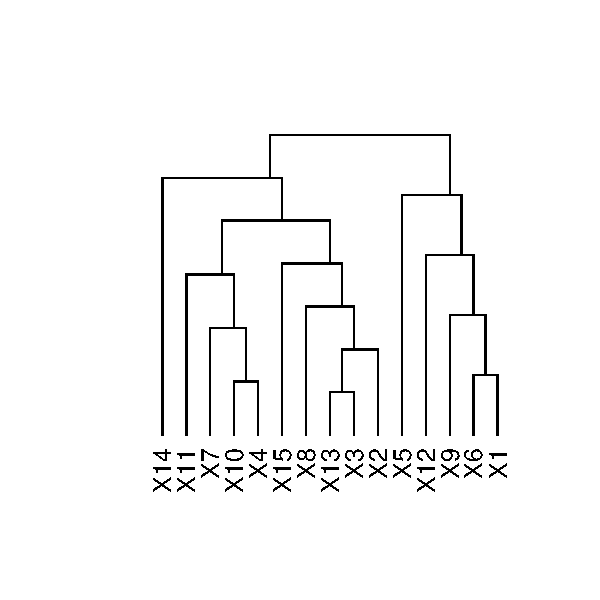
\includegraphics[width=\maxwidth]{figure/dendrograma1-1} 

}

\caption[Clusterización con \texttt{MIN}]{Clusterización con \texttt{MIN}}\label{fig:dendrograma1}
\end{figure}

\end{knitrout}
		 		}
		 		{\small
\begin{knitrout}
\definecolor{shadecolor}{rgb}{0.969, 0.969, 0.969}\color{fgcolor}\begin{kframe}
\begin{alltt}
\hlkwd{fcd_ahc}\hlstd{(sample,} \hlstr{"MAX"}\hlstd{)}
\end{alltt}
\begin{verbatim}
## 
## 
## Matriz cofenética
##           X1        X2        X3       X4       X5        X6       X7       X8
## 1  0.0000000        NA        NA       NA       NA        NA       NA       NA
## 2  4.5961941 0.0000000        NA       NA       NA        NA       NA       NA
## 3  4.5961941 0.7905694 0.0000000       NA       NA        NA       NA       NA
## 4  4.5961941 2.8504386 2.8504386 0.000000       NA        NA       NA       NA
## 5  1.0606602 4.5961941 4.5961941 4.596194 0.000000        NA       NA       NA
## 6  0.2500000 4.5961941 4.5961941 4.596194 1.060660 0.0000000       NA       NA
## 7  4.5961941 2.8504386 2.8504386 0.500000 4.596194 4.5961941 0.000000       NA
## 8  4.5961941 0.5590170 0.7905694 2.850439 4.596194 4.5961941 2.850439 0.000000
## 9  0.3535534 4.5961941 4.5961941 4.596194 1.060660 0.3535534 4.596194 4.596194
## 10 4.5961941 3.4003676 3.4003676 3.400368 4.596194 4.5961941 3.400368 3.400368
## 11 4.5961941 3.4003676 3.4003676 3.400368 4.596194 4.5961941 3.400368 3.400368
## 12 0.9013878 4.5961941 4.5961941 4.596194 1.060660 0.9013878 4.596194 4.596194
## 13 4.5961941 2.8504386 2.8504386 2.573908 4.596194 4.5961941 2.573908 2.850439
## 14 4.5961941 3.4003676 3.4003676 3.400368 4.596194 4.5961941 3.400368 3.400368
## 15 4.5961941 2.8504386 2.8504386 2.474874 4.596194 4.5961941 2.474874 2.850439
##           X9       X10      X11      X12      X13      X14 X15
## 1         NA        NA       NA       NA       NA       NA  NA
## 2         NA        NA       NA       NA       NA       NA  NA
## 3         NA        NA       NA       NA       NA       NA  NA
## 4         NA        NA       NA       NA       NA       NA  NA
## 5         NA        NA       NA       NA       NA       NA  NA
## 6         NA        NA       NA       NA       NA       NA  NA
## 7         NA        NA       NA       NA       NA       NA  NA
## 8         NA        NA       NA       NA       NA       NA  NA
## 9  0.0000000        NA       NA       NA       NA       NA  NA
## 10 4.5961941 0.0000000       NA       NA       NA       NA  NA
## 11 4.5961941 0.7071068 0.000000       NA       NA       NA  NA
## 12 0.9013878 4.5961941 4.596194 0.000000       NA       NA  NA
## 13 4.5961941 3.4003676 3.400368 4.596194 0.000000       NA  NA
## 14 4.5961941 1.2500000 1.250000 4.596194 3.400368 0.000000  NA
## 15 4.5961941 3.4003676 3.400368 4.596194 2.573908 3.400368   0
## 
## Dendrograma final
##                     levelName
## 1  C14                       
## 2   ¦--C13                   
## 3   ¦   ¦--C9                
## 4   ¦   ¦   ¦--X14           
## 5   ¦   ¦   °--C5            
## 6   ¦   ¦       ¦--X11       
## 7   ¦   ¦       °--X10       
## 8   ¦   °--C12               
## 9   ¦       ¦--C11           
## 10  ¦       ¦   ¦--X13       
## 11  ¦       ¦   °--C10       
## 12  ¦       ¦       ¦--X15   
## 13  ¦       ¦       °--C3    
## 14  ¦       ¦           ¦--X7
## 15  ¦       ¦           °--X4
## 16  ¦       °--C6            
## 17  ¦           ¦--X3        
## 18  ¦           °--C4        
## 19  ¦               ¦--X8    
## 20  ¦               °--X2    
## 21  °--C8                    
## 22      ¦--X5                
## 23      °--C7                
## 24          ¦--X12           
## 25          °--C2            
## 26              ¦--X9        
## 27              °--C1        
## 28                  ¦--X6    
## 29                  °--X1    
## 
## 
## Coeficiente de CPCC:  0.8157924
\end{verbatim}
\end{kframe}\begin{figure}

{\centering 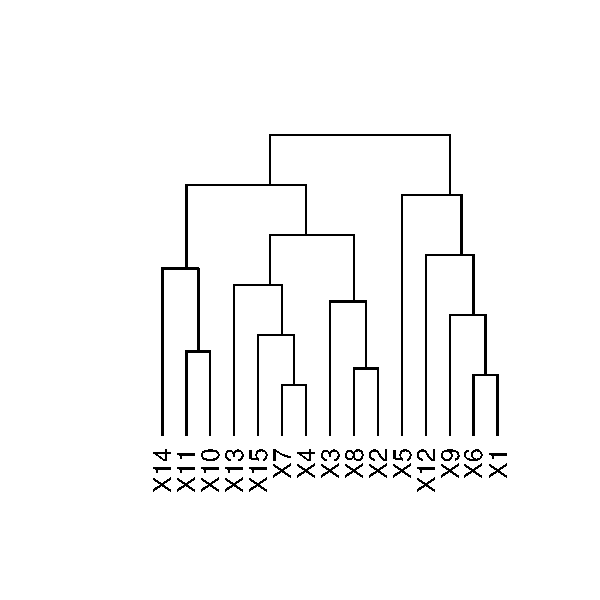
\includegraphics[width=\maxwidth]{figure/dendrograma2-1} 

}

\caption[Clusterización con \texttt{MAX}]{Clusterización con \texttt{MAX}}\label{fig:dendrograma2}
\end{figure}

\end{knitrout}
		 		}
		 		{\small
\begin{knitrout}
\definecolor{shadecolor}{rgb}{0.969, 0.969, 0.969}\color{fgcolor}\begin{kframe}
\begin{alltt}
\hlkwd{fcd_ahc}\hlstd{(sample,} \hlstr{"AVG"}\hlstd{)}
\end{alltt}
\begin{verbatim}
## 
## 
## Matriz cofenética
##           X1        X2        X3        X4        X5        X6        X7
## 1  0.0000000        NA        NA        NA        NA        NA        NA
## 2  3.6662879 0.0000000        NA        NA        NA        NA        NA
## 3  3.6662879 0.4110307 0.0000000        NA        NA        NA        NA
## 4  3.6662879 2.6284228 2.6284228 0.0000000        NA        NA        NA
## 5  0.7297887 3.6662879 3.6662879 3.6662879 0.0000000        NA        NA
## 6  0.2500000 3.6662879 3.6662879 3.6662879 0.7297887 0.0000000        NA
## 7  3.6662879 2.6284228 2.6284228 0.4267767 3.6662879 3.6662879 0.0000000
## 8  3.6662879 0.5590170 0.4110307 2.6284228 3.6662879 3.6662879 2.6284228
## 9  0.3017767 3.6662879 3.6662879 3.6662879 0.7297887 0.3017767 3.6662879
## 10 3.6662879 2.6284228 2.6284228 0.3535534 3.6662879 3.6662879 0.4267767
## 11 3.6662879 2.6284228 2.6284228 0.6170765 3.6662879 3.6662879 0.6170765
## 12 0.7225039 3.6662879 3.6662879 3.6662879 0.7297887 0.7225039 3.6662879
## 13 3.6662879 0.4110307 0.5000000 2.6284228 3.6662879 3.6662879 2.6284228
## 14 3.6662879 2.6284228 2.6284228 0.8173555 3.6662879 3.6662879 0.8173555
## 15 3.6662879 0.7066960 0.7066960 2.6284228 3.6662879 3.6662879 2.6284228
##           X8        X9       X10       X11      X12      X13      X14 X15
## 1         NA        NA        NA        NA       NA       NA       NA  NA
## 2         NA        NA        NA        NA       NA       NA       NA  NA
## 3         NA        NA        NA        NA       NA       NA       NA  NA
## 4         NA        NA        NA        NA       NA       NA       NA  NA
## 5         NA        NA        NA        NA       NA       NA       NA  NA
## 6         NA        NA        NA        NA       NA       NA       NA  NA
## 7         NA        NA        NA        NA       NA       NA       NA  NA
## 8  0.0000000        NA        NA        NA       NA       NA       NA  NA
## 9  3.6662879 0.0000000        NA        NA       NA       NA       NA  NA
## 10 2.6284228 3.6662879 0.0000000        NA       NA       NA       NA  NA
## 11 2.6284228 3.6662879 0.6170765 0.0000000       NA       NA       NA  NA
## 12 3.6662879 0.7225039 3.6662879 3.6662879 0.000000       NA       NA  NA
## 13 0.4110307 3.6662879 2.6284228 2.6284228 3.666288 0.000000       NA  NA
## 14 2.6284228 3.6662879 0.8173555 0.8173555 3.666288 2.628423 0.000000  NA
## 15 0.7066960 3.6662879 2.6284228 2.6284228 3.666288 0.706696 2.628423   0
## 
## Dendrograma final
##                      levelName
## 1  C14                        
## 2   ¦--C13                    
## 3   ¦   ¦--C12                
## 4   ¦   ¦   ¦--X14            
## 5   ¦   ¦   °--C8             
## 6   ¦   ¦       ¦--X11        
## 7   ¦   ¦       °--C4         
## 8   ¦   ¦           ¦--X7     
## 9   ¦   ¦           °--C3     
## 10  ¦   ¦               ¦--X10
## 11  ¦   ¦               °--X4 
## 12  ¦   °--C9                 
## 13  ¦       ¦--X15            
## 14  ¦       °--C7             
## 15  ¦           ¦--C5         
## 16  ¦           ¦   ¦--X13    
## 17  ¦           ¦   °--X3     
## 18  ¦           °--C6         
## 19  ¦               ¦--X8     
## 20  ¦               °--X2     
## 21  °--C11                    
## 22      ¦--X5                 
## 23      °--C10                
## 24          ¦--X12            
## 25          °--C2             
## 26              ¦--X9         
## 27              °--C1         
## 28                  ¦--X6     
## 29                  °--X1     
## 
## 
## Coeficiente de CPCC:  0.9423605
\end{verbatim}
\end{kframe}\begin{figure}

{\centering 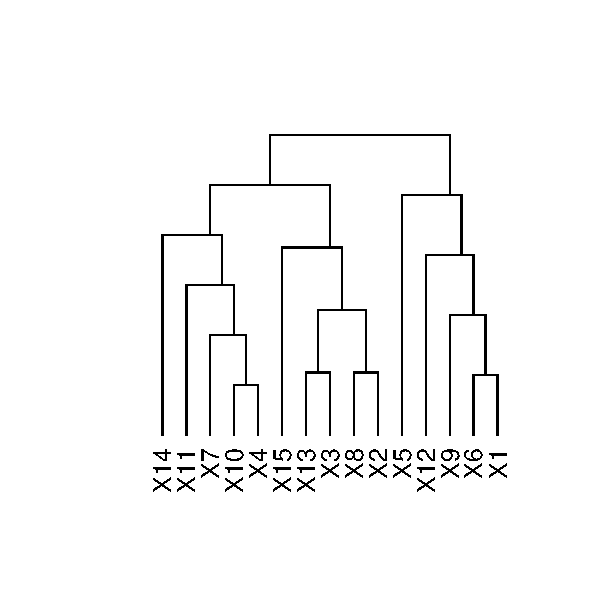
\includegraphics[width=\maxwidth]{figure/dendrograma3-1} 

}

\caption[Clusterización con \texttt{AVG}]{Clusterización con \texttt{AVG}}\label{fig:dendrograma3}
\end{figure}

\end{knitrout}
		 		}
				 
 		\section{Clasificación supervisada}
 		
 			\subsection{Árboles de decisión}
 			
 				\begin{exercise}
 					El tercer conjunto de datos, que se empleará para realizar el análisis de clasificación supervisada utilizando árboles de decisión, estará formado por el siguiente conjunto de 10 sucesos constituidos por los valores de cuatro características de vehículos: 1. \{B, 4, 5, Coche\}; 2. \{A, 2, 2, Moto\}; 3. \{N, 2, 1, Bicicleta\}; 4. \{B, 6, 4, Camión\};
 					5. \{B, 4, 6, Coche\}; 6. \{B, 4, 4, Coche\}; 7.\{N, 2, 2, Bicicleta\}; 8. \{B, 2, 1, Moto\}; 9. \{B, 6, 2, Camión\}; 10. \{N, 2, 1, Bicicleta\}, donde las características de cada suceso son: \{TipoCarnet, NúmeroRuedas, NúmeroPasajeros, TipoVehículo\}. Se debe clasificar el tipo de vehículo en función del resto de características. TipoCarnet, es el
 					tipo de carnet necesario para conducir el vehículo.
 				\end{exercise}
 				
 				Para este conjunto de datos se va a plantear un estudio de clasificación supervisada utilizando como técnica los árboles de decisión. Se buscará definir, a partir de la muestra, un modelo de clasificación que permita obtener el valor de una característica a partir del valor del resto de características. \\
 				
 				Como se necesita una muestra, lo primero que se va a realizar es la lectura del fichero Excel (\texttt{.xlsx}) por medio de la función \texttt{read.xlsx} del paquete \texttt{openxlsx}. Al igual que en el resto de ejercicios, se deberá pasar la ruta del fichero. En él se encuentra contenido el conjunto de daos propuesto para el ejercicio.
 				
\begin{knitrout}
\definecolor{shadecolor}{rgb}{0.969, 0.969, 0.969}\color{fgcolor}\begin{kframe}
\begin{alltt}
\hlstd{(sample} \hlkwb{=} \hlkwd{read.xlsx}\hlstd{(}\hlstr{"data/vehiculos.xlsx"}\hlstd{))}
\end{alltt}
\begin{verbatim}
##    tCarnet nRuedas nPasajeros tVehículo
## 1        B       4          5     Coche
## 2        A       2          2      Moto
## 3        N       2          1 Bicicleta
## 4        B       6          4    Camión
## 5        B       4          6     Coche
## 6        B       4          4     Coche
## 7        N       2          2 Bicicleta
## 8        B       2          1      Moto
## 9        B       6          2    Camión
## 10       N       2          1 Bicicleta
\end{verbatim}
\end{kframe}
\end{knitrout}
 				
 				Una vez tenemos los datos leídos hay que plantear el problema. En este caso, se pretende sacar el tipo de vehículo (\texttt{tVehiculo}) a partir del resto de características (\texttt{tCarnet}, \texttt{nRuedas} y \texttt{nPasajeros}). Al primero le llamaremos a partir de ahora clasificador. Se va a hacer uso del algoritmo de Hunt. Este algoritmo de clasificación supervisada basada en árboles de decisión se compone de dos pasos fundamentales:
 				
 				\begin{enumerate}[label = \textbf{\arabic*.}]
 					\item \textbf{Selección de nodo}: Para el primer paso se elige una característica, que compondrá la raíz del árbol. En el resto de pasos, esta selección formará los nodos intermedios del mismo. La característica que forme el nodo nunca podrá ser el clasificador (\texttt{tVehiculo} en este caso). El objetivo de este árbol, una vez formado, es ver en cada nodo una característica. De cada nodo saldrán hijos cuya diferencia será el valor de la característica del nodo padre. Los hijos contendrán, o bien un valor del clasificador (lo que permitirá clasificar directamente un suceso de la muestra), o bien un subárbol del que dependerá la clasificación del resto de la muestra (habrá que recorrerlo para poder clasificar un suceso de la muestra). 
 					
 					Con el fin de poder optimizar estos árboles, se ha de encontrar la característica que mejor clasifique en base a la muestra con la que se está trabajando. Esto se va a realizar con la medida de ganancia de información ($\Delta_I$). Esta medida mide de una división, la diferencia de impureza entre el nodo padre y los nodos hijos una vez realizada esa división. A mayor ganancia de información, mejor división se habrá realizado, por lo que el objetivo será implementar a la clasificación la división con mayor $\Delta_I$. La ganancia de información se calcula de la siguiente forma:
 					
 					
					$$
					\Delta_i = I_{\text{padre}} - \sum_{j=1}^k \frac{N(n_j)}{N} \cdot I(n_j)
					$$
 					
 					\begin{itemize}
 						\item $I_{\text{padre}}$: Impureza del nodo padre
 						\item $k$: Número total de hijos (en esta implementación siempre será 2)
 						\item $N(n_j)$: Número de sucesos de la muestra asociados al nodo hijo $j$
 						\item $N$: Número total de sucesos de la muestra actual
 						\item $I(n_j)$: Impureza del nodo hijo $j$
 					\end{itemize}
 					
 					Como se puede ver, para calcular la ganancia de información, se necesita la impureza $I$ del nodo padre y de sus hijos. Esta puede ser calculada de diferentes formas en función del método que se utilice. Todas ellas utilizan las frecuencias relativas ($f_i$) de las clases de equivalencia $c$ del clasificador. Se distinguen tres:
 					
 					\begin{itemize}
 						\item \textbf{Entropía}
 						$$
 						I= - \sum_{i=1}^{c} f_i\log_{c}(f_i)
 						$$
 								
 						\item \textbf{Error}
						$$
						I = 1 - \max\{f_i\}_{i=1}^c
						$$
 						
 						\item \textbf{Gini}
						$$
						I = 1 - \sum_{i=1}^{c} f_i^2
						$$
 					\end{itemize}
 					
 					\item \textbf{Clasificación de los sucesos:} Una vez se ha elegido la característica que va a conformar el nodo, se clasifica. Si se pueden clasificar completamente los sucesos de la muestra (que en cada hijo solo haya un valor del clasificador posible) se trata de un nodo final y termina la clasificación. Si no lo permite, se trata de un nodo interno, por lo que hay que volver al primer paso.  
 					
 					Una observación a tener en cuenta es que un nodo ha clasificado completamente cuando la impureza del padre es igual a la ganancia de información ($\Delta_I = I_{\text{padre}}$), ya que significa que las impurezas de los hijos son 0. Cada vez que se clasifique con un criterio determinado, todas las filas de la muestra que contengan ese o esos valores en la característica del nodo se deben eliminar (ya que se considera que han sido clasificadas). 
 					
 					Puede darse el caso en el que el algoritmo no pueda seguir clasificando porque la ganancia de información sea 0 en todos los escenarios de clasificación posibles. En ese caso, el algoritmo finalizará habiendo clasificado todo lo anterior pero dejando el nodo final abierto, es decir, sin una clasificación concreta.
 					
 				\end{enumerate}
 				
 				En esta implementación se utilizarán árboles binarios (cada nodo con 2 hijos) tal y como se ha mencionado previamente. Esto condiciona la forma de actuar en el algoritmo, así que la metodología a seguir se resume en los siguientes pasos:
 				
 				\begin{enumerate}
 					\item \textbf{Selección del mejor nodo}: Se realizará la clasificación en base a 
 					\item \textbf{Unión de la clasificación actual al resto de clasificación}:
 					\item \textbf{Recorte de la muestra}:
 				\end{enumerate}
 				
 				Estos paso se realizarán hasta que el algoritmo finalice. Este finalizará atendiendo a las siguientes condiciones:
 				
 				
 				Con esta base teórica se procede a explicar la implementación del algoritmo en R. En primer lugar...
 			\subsection{Regresión lineal}
 			
 				\begin{exercise}
 					El cuarto conjunto de datos, que se empleará para realizar el análisis de clasificación supervisada utilizando regresión, estará formado por los siguientes 4 subconjuntos de datos: 1. \{10, 8.04; 8, 6.95; 13, 7.58; 9, 8.81; 11, 8.33; 14, 9.96; 6, 7.24; 4, 4.26; 12, 10.84; 7, 4.82; 5, 5.68\}; 2. \{10, 9.14; 8, 8.14; 13, 8.74; 9, 8.77; 11, 9.26; 14, 8.1; 6, 6.13; 4, 3.1; 12, 9.13; 7, 7.26; 5, 4.74\}; 3. \{10, 7.46; 8, 6.77; 13, 12.74; 9, 7.11; 11, 7.81; 14, 8.84; 6, 6.08; 4, 5.39; 12, 8.15; 7, 6.42; 5, 5.73\}; 4. \{8, 6.58; 8, 5.76; 8, 7.71; 8, 8.84; 8, 8.47; 8, 7.04; 8, 5.25; 19, 12.5; 8, 5.56; 8, 7.91; 8, 6.89\}. Se deben calcular las rectas de regresión de los cuatro subconjuntos y sus parámetros de ajuste.
 				\end{exercise}
 				
 				Para la resolución de este ejercicio, se hará uso de la recta de regresión lineal de la forma $\hat{y} = a + bx$ donde los parámetros $a$ y $b$ obedecen a las siguiente ecuaciones. 
 				
 				\begin{equation}\label{ec:reg_param}
 					\begin{gathered}
 						b = \frac{S_{xy}}{S^2_x}\\
 						a = \bar{y} - b \bar{x}
 					\end{gathered}
 				\end{equation}
 				
 				Para el cálculo de estos parámetros se necesita hacer uso de funciones ya implementadas en la práctica anterior como la media aritmética, la desviación típica y la varianza, se recuerda el código a continuación. 
 				
\begin{knitrout}
\definecolor{shadecolor}{rgb}{0.969, 0.969, 0.969}\color{fgcolor}\begin{kframe}
\begin{alltt}
\hlstd{fcd_mean} \hlkwb{=} \hlkwa{function}\hlstd{(}\hlkwc{list}\hlstd{) \{}
        \hlstd{add} \hlkwb{=} \hlnum{0}
        \hlkwa{for} \hlstd{(i} \hlkwa{in} \hlnum{1}\hlopt{:}\hlkwd{len}\hlstd{(list)) \{}
                \hlstd{add} \hlkwb{=} \hlstd{add} \hlopt{+} \hlstd{list[i]}
        \hlstd{\}}
        \hlstd{add} \hlopt{/} \hlkwd{len}\hlstd{(list)}
\hlstd{\}}

\hlstd{standard_dev} \hlkwb{=} \hlkwa{function}\hlstd{(}\hlkwc{list}\hlstd{) \{}
        \hlstd{mean} \hlkwb{=} \hlkwd{fcd_mean}\hlstd{(list)}
        \hlstd{n} \hlkwb{=} \hlkwd{len}\hlstd{(list)}
        \hlstd{add} \hlkwb{=} \hlnum{0}
        \hlkwa{for} \hlstd{(i} \hlkwa{in} \hlnum{1}\hlopt{:}\hlstd{n) \{}
                \hlstd{add} \hlkwb{=} \hlstd{add} \hlopt{+} \hlstd{((list[i]} \hlopt{-} \hlstd{mean)}\hlopt{^}\hlnum{2}\hlstd{)}
        \hlstd{\}}
        \hlkwd{sqrt}\hlstd{(add}\hlopt{/}\hlstd{n)}
\hlstd{\}}

\hlstd{variance} \hlkwb{=} \hlkwa{function}\hlstd{(}\hlkwc{list}\hlstd{) \{}
        \hlstd{dev} \hlkwb{=} \hlkwd{standard_dev}\hlstd{(list)}
        \hlstd{var} \hlkwb{=} \hlstd{dev}\hlopt{^}\hlnum{2}
        \hlstd{var}
\hlstd{\}}
\end{alltt}
\end{kframe}
\end{knitrout}
 				
 				El siguiente cálculo será hallar el valor de la covarianza de la siguiente manera
 				
 				\begin{equation}\label{ec:reg_cov}
 					S_{xy} = \frac{\displaystyle\sum_{i=1}^nx_iy_i}{n} - \bar{x}\bar{y}, 
 				\end{equation}
 				
 				y quedará reflejado en la función \texttt{covariance} que recibe dos vectores que representan los datos y sus valores correspondientes: 
 				
 				$$
 				\begin{gathered}
 					\textbf{X} = (x_1, x_2, \hdots, x_n)\\
 					\textbf{Y} = (y_1, y_2, \hdots, y_n)
 				\end{gathered}
 				$$
 				
 				La función realiza el cálculo de la \Cref{ec:reg_cov} usando \texttt{\%*\%}, que en este caso realiza el producto escalar de \textbf{X} e \textbf{Y}. También se verifica que estos vectores compartan dimensiones, pues de lo contrario no se podrá calcular. 
 				
\begin{knitrout}
\definecolor{shadecolor}{rgb}{0.969, 0.969, 0.969}\color{fgcolor}\begin{kframe}
\begin{alltt}
\hlstd{covariance} \hlkwb{=} \hlkwa{function}\hlstd{(}\hlkwc{x}\hlstd{,} \hlkwc{y}\hlstd{) \{}
        \hlkwa{if} \hlstd{(}\hlkwd{len}\hlstd{(x)} \hlopt{!=} \hlkwd{len}\hlstd{(y)) \{}
                \hlkwd{stop}\hlstd{(}\hlstr{"X e Y deben tener la misma dimensión"}\hlstd{)}
        \hlstd{\}}
        \hlkwa{else} \hlstd{\{}
                \hlstd{sum} \hlkwb{=} \hlstd{x} \hlopt \hlstd{y}
                \hlstd{(sum}\hlopt{/}\hlkwd{len}\hlstd{(x))}\hlopt{-}\hlstd{(}\hlkwd{fcd_mean}\hlstd{(x)}\hlopt{*}\hlkwd{fcd_mean}\hlstd{(y))}
        \hlstd{\}}
\hlstd{\}}
\end{alltt}
\end{kframe}
\end{knitrout}
 				
 				Finalmente, la función \texttt{regression\_line} calcula los parámetros $a$ y $b$ mediante la \Cref{ec:reg_param}. Devuelve el resultado de forma matricial para más tarde trabajar de forma más cómoda. 
 				
 				$$
 				\textbf{P} = \begin{pmatrix}
 					a\\
 					b
 				\end{pmatrix}
 				$$
 				
\begin{knitrout}
\definecolor{shadecolor}{rgb}{0.969, 0.969, 0.969}\color{fgcolor}\begin{kframe}
\begin{alltt}
\hlstd{regression_line} \hlkwb{=} \hlkwa{function}\hlstd{(}\hlkwc{x}\hlstd{,} \hlkwc{y}\hlstd{) \{}
        \hlstd{b} \hlkwb{=} \hlkwd{covariance}\hlstd{(x, y)} \hlopt{/} \hlkwd{variance}\hlstd{(x)}
        \hlstd{a} \hlkwb{=} \hlkwd{fcd_mean}\hlstd{(y)} \hlopt{-} \hlstd{b} \hlopt{*} \hlkwd{fcd_mean}\hlstd{(x)}
        \hlkwd{matrix}\hlstd{(}\hlkwd{c}\hlstd{(a, b),} \hlkwc{ncol} \hlstd{=} \hlnum{1}\hlstd{)}
\hlstd{\}}
\end{alltt}
\end{kframe}
\end{knitrout}
 				
 				Una vez se tienen calculados los parámetros de la recta de regresión lineal, es momento de evaluar cómo de buena es la aproximación. Para ello se emplea la métrica $R^2$. Su valor depende de otros dos, $SSR$ y $SSY$, que obedecen a las siguientes ecuaciones. 
 				
 				$$
 				\begin{gathered}
 					SSR = \sum_{i=1}^n(\hat{y}_i - \bar{y})^2\\
 					SSY = \sum_{i=1}^n(y_i - \bar{y})^2
 				\end{gathered}
 				$$
 				
 				Estos cálculos quedan recogidos en las funciones \texttt{ssr} y \texttt{ssy}. La primera de ellas calcula el valor requerido de forma matricial, recibiendo \textbf{P}, \textbf{X}, e \textbf{Y} como parámetros, y realiza las siguientes operaciones, donde el cuadrado se realiza elemento a elemento, en vez de forma matricial. En este caso, \texttt{\%*\%} funciona como el producto de matrices usual. 
 				
 				$$
 				\begin{gathered}
 					\hat{\textbf{Y}} = \begin{pmatrix}
 						1 & x_1\\
 						1 & x_2\\
 						\vdots & \vdots\\
 						1 & x_n
 					\end{pmatrix}\begin{pmatrix}
 						a\\
 						b
 					\end{pmatrix}\\
 					SSR = \sum_{i=1}^n (\hat{\textbf{Y}_i} - \bar{\textbf{Y}}_i)^2
 				\end{gathered}
 				$$
 				
 				De la manera similar, se calcula el $SSY$ como $\sum_{i=1}^n (\textbf{Y}_i - \bar{\textbf{Y}}_i)^2$. Además se conoce que la relación entre estos dos parámetros y $R^2$ es la siguiente. 
 				
 				$$
 				R^2 = \frac{SSR}{SSY}
 				$$
 				
\begin{knitrout}
\definecolor{shadecolor}{rgb}{0.969, 0.969, 0.969}\color{fgcolor}\begin{kframe}
\begin{alltt}
\hlstd{ssr} \hlkwb{=} \hlkwa{function}\hlstd{(}\hlkwc{p}\hlstd{,} \hlkwc{x}\hlstd{,} \hlkwc{y}\hlstd{) \{}
        \hlstd{X} \hlkwb{=} \hlkwd{matrix}\hlstd{(}\hlkwd{c}\hlstd{(}\hlkwd{rep}\hlstd{(}\hlnum{1}\hlstd{,} \hlkwc{times} \hlstd{=} \hlkwd{len}\hlstd{(x)), x),} \hlkwc{ncol} \hlstd{=} \hlnum{2}\hlstd{)}
        \hlstd{y_hat} \hlkwb{=} \hlstd{X} \hlopt \hlstd{p}
        \hlkwd{sum}\hlstd{((y_hat} \hlopt{-} \hlkwd{rep}\hlstd{(}\hlkwd{fcd_mean}\hlstd{(y)))}\hlopt{^}\hlnum{2}\hlstd{)}
\hlstd{\}}

\hlstd{ssy} \hlkwb{=} \hlkwa{function}\hlstd{(}\hlkwc{y}\hlstd{) \{}
        \hlkwd{sum}\hlstd{((y} \hlopt{-} \hlkwd{rep}\hlstd{(}\hlkwd{fcd_mean}\hlstd{(y)))}\hlopt{^}\hlnum{2}\hlstd{)}
\hlstd{\}}

\hlstd{r2} \hlkwb{=} \hlkwa{function}\hlstd{(}\hlkwc{sr}\hlstd{,} \hlkwc{sy}\hlstd{) \{}
        \hlstd{sr}\hlopt{/}\hlstd{sy}
\hlstd{\}}
\end{alltt}
\end{kframe}
\end{knitrout}
 				
 				Finalmente se encapsula todo en una única función llamada \texttt{fcd\_regression} que muestra por consola la ecuación de $\hat{y}$ y el valor de $R^2$, además de una gráfica con la recta y los puntos. 
 				
\begin{knitrout}
\definecolor{shadecolor}{rgb}{0.969, 0.969, 0.969}\color{fgcolor}\begin{kframe}
\begin{alltt}
\hlstd{fcd_regression} \hlkwb{=} \hlkwa{function}\hlstd{(}\hlkwc{sample}\hlstd{) \{}
        \hlstd{X} \hlkwb{=} \hlstd{sample[,} \hlnum{1}\hlstd{]}
        \hlstd{Y} \hlkwb{=} \hlstd{sample[,} \hlnum{2}\hlstd{]}

        \hlstd{param} \hlkwb{=} \hlkwd{regression_line}\hlstd{(X, Y)}
        \hlstd{r} \hlkwb{=} \hlkwd{r2}\hlstd{(}\hlkwd{ssr}\hlstd{(param, X, Y),} \hlkwd{ssy}\hlstd{(Y))}

        \hlstd{a} \hlkwb{=} \hlstd{param[}\hlnum{1}\hlstd{,} \hlnum{1}\hlstd{]}
        \hlstd{b} \hlkwb{=} \hlstd{param[}\hlnum{2}\hlstd{,} \hlnum{1}\hlstd{]}

        \hlkwd{print}\hlstd{(}\hlkwd{sprintf}\hlstd{(}\hlstr{"y = %.3fx + %.3f"}\hlstd{, b, a))}
        \hlkwd{print}\hlstd{(}\hlkwd{sprintf}\hlstd{(}\hlstr{"R2 = %.3f"}\hlstd{, r))}

        \hlkwd{plot}\hlstd{(X, Y,} \hlkwc{col} \hlstd{=} \hlstr{"blue"}\hlstd{,} \hlkwc{main} \hlstd{=} \hlstr{"Recta de regresión"}\hlstd{,}
                \hlkwc{xlab} \hlstd{=} \hlstr{"Eje X"}\hlstd{,} \hlkwc{ylab} \hlstd{=} \hlstr{"Eje Y"}\hlstd{)}
        \hlkwd{abline}\hlstd{(}\hlkwc{a}\hlstd{=a,} \hlkwc{b}\hlstd{=b,} \hlkwc{col}\hlstd{=}\hlstr{"red"}\hlstd{)}
\hlstd{\}}
\end{alltt}
\end{kframe}
\end{knitrout}
 				
 				De la siguiente forma, se prueba para los casos del profesor. Se observa que las aproximaciones no son buenas, pues los valores de $R^2$ no se aproximan a 1. En la \Cref{fig:recta1} se debe a que los puntos se encuentran de manera un tanto dispersa, dando a entender que no existe relación entre las variables. En la \Cref{fig:recta2} se ve claramente que la relación es cuadrática, por lo que es inadecuado utilizar una recta para aproximar esos puntos. En la \Cref{fig:recta3} el problema viene dado por un outlier, y en la \Cref{fig:recta4} se dan diferentes valores a $y$ para un mismo $x$ lo que hace que la pendiente de esta recta tienda a infinito. %explicar la carga de datos
 				
\begin{knitrout}
\definecolor{shadecolor}{rgb}{0.969, 0.969, 0.969}\color{fgcolor}\begin{kframe}
\begin{alltt}
\hlstd{sample1} \hlkwb{=} \hlkwd{read.xlsx}\hlstd{(}\hlstr{"../Memoria/data/conj1.xlsx"}\hlstd{,} \hlkwc{colNames}\hlstd{=}\hlnum{FALSE}\hlstd{)}
\hlkwd{fcd_regression}\hlstd{(sample1)}
\end{alltt}
\begin{verbatim}
## [1] "y = 0.500x + 3.000"
## [1] "R2 = 0.667"
\end{verbatim}
\end{kframe}\begin{figure}

{\centering 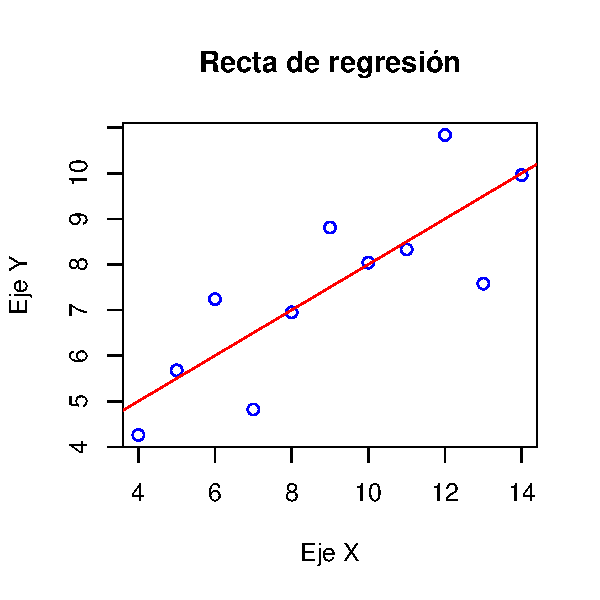
\includegraphics[width=\maxwidth]{figure/recta1-1} 

}

\caption[Datos no correlacionados]{Datos no correlacionados}\label{fig:recta1}
\end{figure}

\end{knitrout}
 				
\begin{knitrout}
\definecolor{shadecolor}{rgb}{0.969, 0.969, 0.969}\color{fgcolor}\begin{kframe}
\begin{alltt}
\hlstd{sample2} \hlkwb{=} \hlkwd{read.xlsx}\hlstd{(}\hlstr{"../Memoria/data/conj2.xlsx"}\hlstd{,} \hlkwc{colNames}\hlstd{=}\hlnum{FALSE}\hlstd{)}
\hlkwd{fcd_regression}\hlstd{(sample2)}
\end{alltt}
\begin{verbatim}
## [1] "y = 0.500x + 3.001"
## [1] "R2 = 0.666"
\end{verbatim}
\end{kframe}\begin{figure}

{\centering 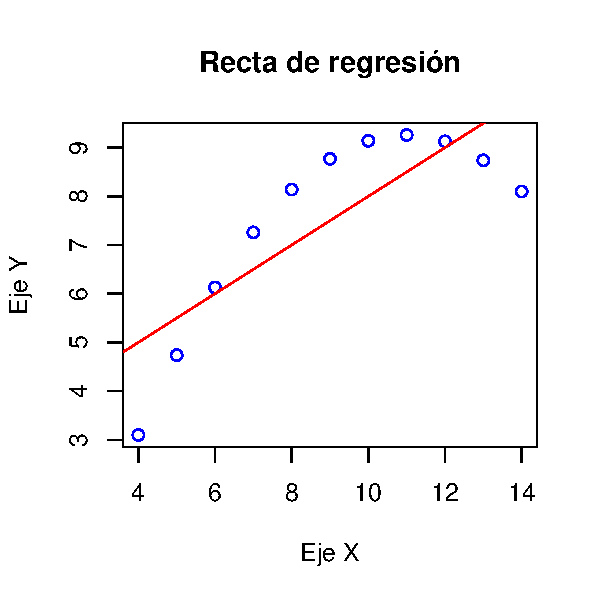
\includegraphics[width=\maxwidth]{figure/recta2-1} 

}

\caption[Relación cuadrática]{Relación cuadrática}\label{fig:recta2}
\end{figure}

\end{knitrout}
 				
\begin{knitrout}
\definecolor{shadecolor}{rgb}{0.969, 0.969, 0.969}\color{fgcolor}\begin{kframe}
\begin{alltt}
\hlstd{sample3} \hlkwb{=} \hlkwd{read.xlsx}\hlstd{(}\hlstr{"../Memoria/data/conj3.xlsx"}\hlstd{,} \hlkwc{colNames}\hlstd{=}\hlnum{FALSE}\hlstd{)}
\hlkwd{fcd_regression}\hlstd{(sample3)}
\end{alltt}
\begin{verbatim}
## [1] "y = 0.500x + 3.002"
## [1] "R2 = 0.666"
\end{verbatim}
\end{kframe}\begin{figure}

{\centering 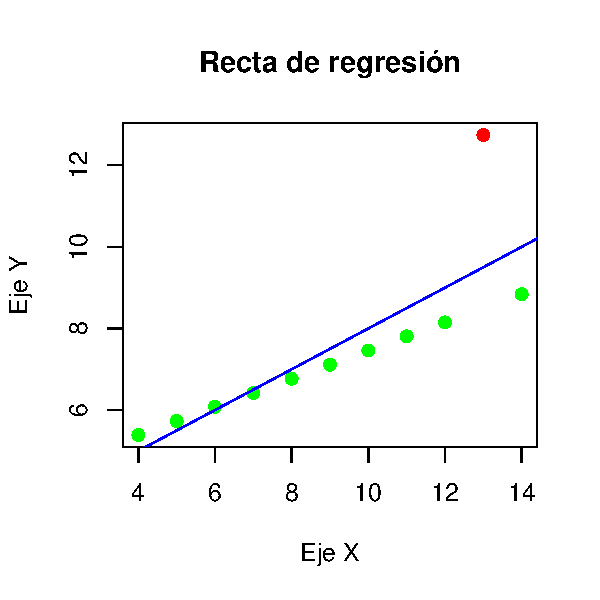
\includegraphics[width=\maxwidth]{figure/recta3-1} 

}

\caption[Relación lineal con outlier]{Relación lineal con outlier}\label{fig:recta3}
\end{figure}

\end{knitrout}
 				
\begin{knitrout}
\definecolor{shadecolor}{rgb}{0.969, 0.969, 0.969}\color{fgcolor}\begin{kframe}
\begin{alltt}
\hlstd{sample4} \hlkwb{=} \hlkwd{read.xlsx}\hlstd{(}\hlstr{"../Memoria/data/conj4.xlsx"}\hlstd{,} \hlkwc{colNames}\hlstd{=}\hlnum{FALSE}\hlstd{)}
\hlkwd{fcd_regression}\hlstd{(sample4)}
\end{alltt}
\begin{verbatim}
## [1] "y = NaNx + NaN"
## [1] "R2 = NaN"
\end{verbatim}


{\ttfamily\noindent\bfseries\color{errorcolor}{\#\# Error in int\_abline(a = a, b = b, h = h, v = v, untf = untf, ...): 'a' y 'b' deben ser finitos}}\end{kframe}\begin{figure}

{\centering 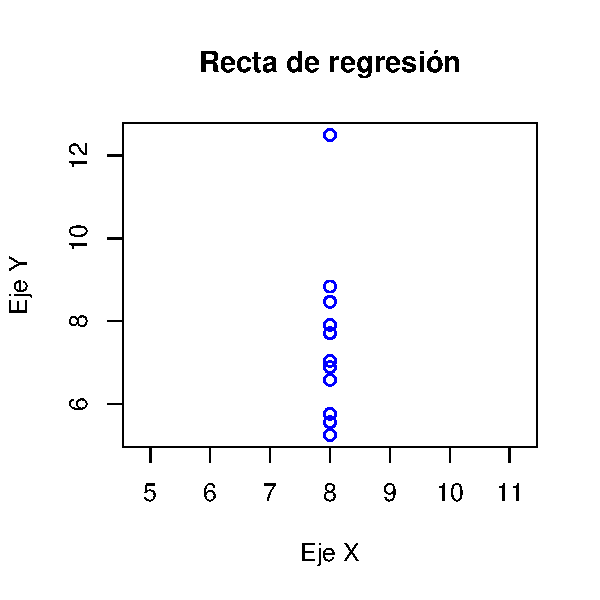
\includegraphics[width=\maxwidth]{figure/recta4-1} 

}

\caption[Recta con pendiente infinita]{Recta con pendiente infinita}\label{fig:recta4}
\end{figure}

\end{knitrout}
 				
\end{document}
